\chapter{代数曲线}\label{ch:1}

\begin{quote}\small\itshape
{\emergencystretch=3em 由此可见，许多有趣的曲线都可以定义为方程 $f(x,y)=0$ 的零点集，其中 $f(x,y)$ 是关于 $x$ 与 $y$ 的多项式. Leibniz 将这样的曲线称为代数曲线.\par}
\end{quote}
\vspace{-0.5em}
\hfill \small \cite[p.~78]{brieskorn1986}.

在本章中, 我们建立代数曲线 (algebraic curves) 的一些基本理论, 重点讨论平面曲线. 在第 \ref{sec:1.3} 节中, 我们将描述三次曲线上自然的群结构.

\section{平面代数曲线；Bezout 定理}\label{sec:1.1}

我们引入平面代数曲线, 并发展平面中曲线的相交理论 (intersection theory).

\subsection*{多项式环}

我们需要用到如下事实: 域上的多项式环是唯一分解整环 (unique factorization domain). 其证明可对变元个数作归纳, 从 ``若环 $A$ 是唯一分解整环, 则多项式环 $A[X]$ 亦然'' (\cite[4.9]{milne-ca}) 这一事实出发. 由于 $k[X_1,\dots,X_n]$ 中的可逆元恰为那些非零常数, 环中任一元素 $f$ 均可写成
\[
f = f_1^{m_1}\dots f_r^{m_r}
\]
的形式, 其中 $f_i$ 是两两互不非常数倍数的不可约多项式 (irreducible polynomials), 且分解在相差常数的意义下唯一. 那些满足 $m_i > 1$ 的 $f_i$ 称为 $f$ 的重复因子 (repeated factors).\index{chongfuyinzi@重复因子(repeated factor)} 多项式 $f$ 不可约当且仅当主理想 $(f)$ 为素理想 (\cite[4.1]{milne-ca}).

\subsection*{仿射平面曲线}

$k$ 上的仿射平面 (affine plane) 是 $\mathbb{A}^2(k) = k\times k$. 一个非常数的多项式 $f\in k[X,Y]$, 假定它在 $k^{\mathrm{al}}[X,Y]$ 中没有重复因子, 定义了 $k$ 上的一条仿射平面曲线 (affine plane curve)\index{fangshepingmianquxian@仿射平面曲线(affine plane curve)} $C_f$, 它在任一包含 $k$ 的域 $K$ 中的点集, 由 $f$ 在 $K^2$ 中的零点给出：
\[
C_f(K) = \{(x,y)\in K^2 \mid f(x,y) = 0\}.
\]
对 $c\in k^{\times}$, 曲线 $C_f$ 与 $C_{cf}$ 在每一个域 $K$ 中都有相同的点, 我们不对它们加以区分.

对定义在 $k$ 上的曲线, 坐标属于 $k$ 的点通常称为曲线上的有理点 ($k$-rational point).\index{youlidian@有理点(rational point)}

若 $f$ 在 $k[X,Y]$ 中不可约, 则称 $C_f$ 不可约 (irreducible)\index{bukeyuequxian@不可约曲线(irreducible curve)}; 若 $f$ 在 $k^{\mathrm{al}}[X,Y]$ 中仍然不可约, 则称 $C_f$ 几何不可约 (geometrically irreducible).\index{jihebukeyuequxian@几何不可约曲线(geometrically irreducible curve)} 对一般的曲线 $C_f$, 可将 $f$ 写成 $f = f_1f_2\cdots f_r$, 其中 $f_i$ 为 $k[X,Y]$ 中两两不同的不可约多项式, 于是
\[
C_f(K) = C_{f_1}(K) \cup \cdots \cup C_{f_r}(K), \qquad \text{对所有 } K\supset k.
\]
曲线 $C_{f_i}$ 称为 $C_f$ 的不可约分支 (irreducible components, 或简称为分支).\index{bukeyuefenzhi@不可约分支(irreducible component)}

记号 $C\colon f=0$ 表示 $C$ 是曲线 $C_f$; 记号 $C\colon f_1=f_2$ 表示 $C$ 是曲线 $C_{f_1-f_2}$.

\begin{example} \label{thm:1.1.1} 
曲线 $X^2 - 2Y^2 = 0$ 在 $\mathbb{Q}$ 上不可约, 但在 $\mathbb{Q}[\sqrt{2}]$ 上分解成两条直线 $(X-\sqrt{2}Y)(X+\sqrt{2}Y)=0$. 因此它不几何不可约.
\end{example}

回忆在特征 $p\neq 0$ 时, 二项式定理给出
\[
(X+Y)^p = X^p + Y^p.
\]

\begin{example} \label{thm:1.1.2} 
若域 $k$ 不是完美域 (perfect field), 则其特征 $\operatorname{char}(k) = p\neq 0$, 且存在 $a\in k$ 不是 $k$ 中的 $p$ 次幂. 该元素 $a$ 在 $k^{\mathrm{al}}$ 中成为 $p$ 次幂, 设 $a = \alpha^p$. 多项式 $f = X^p + aY^p$ 在 $k[X,Y]$ 中不可约, 但在 $k^{\mathrm{al}}[X,Y]$ 中成为纯幂 $f = (X+\alpha Y)^p$, 因此按我们的定义它不构成仿射平面曲线. 此现象只出现在非完美域上. 当 $k$ 为完美域时, 在 $k[X,Y]$ 中无重复因子的多项式在 $k^{\mathrm{al}}[X,Y]$ 中不会获得重复因子.
\end{example}

我们用明显的公式定义多项式的偏导数：
\[
\frac{\partial}{\partial X}\Bigl(\sum_{i,j} a_{ij}X^iY^j\Bigr) = \sum_{i,j} i\,a_{ij}X^{i-1}Y^j.
\]
把 $f(X,Y)$ 写成关于 $X-a$ 和 $Y-b$ 的多项式, 我们得到
\[
f(X,Y) = f(a,b) + \Bigl(\frac{\partial f}{\partial X}\Bigr)(a,b)\,(X-a) + \Bigl(\frac{\partial f}{\partial Y}\Bigr)(a,b)\,(Y-b) + \text{关于 } X-a,\,Y-b \text{ 的次数 }\ge 2 \text{ 的项}.
\]
这称为 $f$ 的泰勒展开 (Taylor expansion\index{Taylor-zhankai@Taylor 展开(Taylor expansion)}\index{Taylor}).

设 $P = (a,b)\in C_f(K)$, 其中 $K\supset k$. 若偏导数 $\frac{\partial f}{\partial X}$ 与 $\frac{\partial f}{\partial Y}$ 在 $P$ 处至少有一个非零, 则称 $P$ 非奇异 (nonsingular)\index{feiqiyi@非奇异(nonsingular)}, 并把 $C$ 在 $P$ 处的切线 (tangent line)\index{qiexian@切线(tangent line)} 定义为
\[
\Bigl(\frac{\partial f}{\partial X}\Bigr)_P (X-a) + \Bigl(\frac{\partial f}{\partial Y}\Bigr)_P (Y-b) = 0.
\]
若 $C(k^{\mathrm{al}})$ 中所有点都非奇异, 则称曲线 $C$ 非奇异 (nonsingular), 否则称其奇异 (singular).\index{qiyi@奇异(singular)}

\begin{aside} \label{thm:1.1.3} 
设 $f(x,y)$ 是 $\mathbb{R}^2$ 上的实值函数. 偏导数至少一个非零的条件意味着曲线在 $P$ 附近有局部参数化. 梯度 $\nabla f \overset{\text{def}}{=} \bigl(\frac{\partial f}{\partial X}, \frac{\partial f}{\partial Y}\bigr)$ 是 $\mathbb{R}^2$ 上的向量场, 其在 $P = (a,b)$ 处的值 $(\nabla f)_P$ 垂直于经过 $P$ 的等值线 $f(x,y) = c$, 故
\[
(\nabla f)_P \cdot (x-a, y-b) = 0
\]
正是等值线的切线方程. 这解释了上述定义.
\end{aside}

\begin{remark} \label{thm:1.1.4} 
\begin{enumerate}[label=\textup{(\alph*)}]
\item 若 $C$ 非奇异, 则对任意包含 $k$ 的域 $K$, $C(K)$ 中的每一点都非奇异. 否则多项式 $f$, $\frac{\partial f}{\partial X}$, $\frac{\partial f}{\partial Y}$ 将生成 $k[X,Y]$ 的真理想, 由零点定理 (Nullstellensatz) 它们在 $k^{\mathrm{al}}$ 中有公共零点.%
\footnote{零点定理说: 若 $f_1,\dots,f_r\in k[X_1,\dots,X_n]$ 生成的理想 $(f_1,\dots,f_r) \neq k[X_1,\dots,X_n]$, 则它们在 $k^{\mathrm{al}}$ 中有公共零点. 见 \cite[13.8]{milne-ca}.}
\item 曲线的两个不可约分支的交点必为奇异点. 例如考虑 $C_f$, 其中 $f = f_1f_2$ 且 $f_1(0,0) = 0 = f_2(0,0)$. 则
\[
\frac{\partial f}{\partial X}(0,0) = \Bigl(f_1\frac{\partial f_2}{\partial X} + \frac{\partial f_1}{\partial X}f_2\Bigr)(0,0) = 0,
\qquad
\frac{\partial f}{\partial Y}(0,0) = \Bigl(f_1\frac{\partial f_2}{\partial Y} + \frac{\partial f_1}{\partial Y}f_2\Bigr)(0,0) = 0,
\]
故 $P = (0,0)$ 是 $C_f$ 的奇异点.
\item 若 $C_f$ 与 $C_g$ 是 $k$ 上无公共分支的仿射平面曲线, 则 $C_f(k^{\mathrm{al}})\cap C_g(k^{\mathrm{al}})$ 有限. 结式理论 (I\ref{thm:1.1.22}, \ref{thm:1.1.24}) 表明, 存在多项式 $a(X,Y)$, $b(X,Y)$, $r(X)$ 使
\[
a(X,Y)F(X,Y) + b(X,Y)G(X,Y) = r(X),
\]
且 $r(x_0) = 0$ 当且仅当 $F(x_0,Y)$ 与 $G(x_0,Y)$ 有公共零点. 多项式 $r(X)$ 只有有限个根, 而对其每个根 $x_0$, $F(x_0,Y)$ 与 $G(x_0,Y)$ 只有有限个公共零点.
\item 设 $f\in k[X,Y]$ 为无重复因子的非常数多项式. 若 $\frac{\partial f}{\partial X}$ 为零多项式, 则要么 $X$ 不出现在 $f$ 中, 要么 $\operatorname{char}(k) = p\neq 0$ 且 $f\in k[X^p,Y]$. 若 $\frac{\partial f}{\partial X}$ 与 $\frac{\partial f}{\partial Y}$ 均为零多项式, 则 $\operatorname{char}(k) = p\neq 0$ 且 $f\in k[X^p,Y^p]$, 即 $f(X,Y) = \sum_{i,j} a_{ij}X^{ip}Y^{jp}$. 若 $k$ 完美, 则
\[
\sum_{i,j} a_{ij}X^{ip}Y^{jp} = \Bigl(\sum_{i,j} a_{ij}^{1/p}X^iY^j\Bigr)^p,
\]
于是 $f$ 是 $k[X,Y]$ 中的 $p$ 次幂, 与对 $f$ 的假设矛盾. 因此, 若 $k$ 完美, 则 $\frac{\partial f}{\partial X}$ 与 $\frac{\partial f}{\partial Y}$ 不同时为零多项式, 且 $C_f(k^{\mathrm{al}})$ 中只有有限个奇异点.
\end{enumerate}
\end{remark}

\begin{example} \label{thm:1.1.5} 
考虑曲线
\[
C\colon Y^2 = X^3 + aX + b.
\]
在 $C$ 的奇异点 $(x,y)$ 处,
\[
2Y = 0, \qquad 3X^2 + a = 0, \qquad Y^2 = X^3 + aX + b.
\]
若 $\operatorname{char}(k)\neq 2$, 则 $y = 0$ 且 $x$ 是 $X^3+aX+b$ 及其导数的公共根, 即 $x$ 是 $X^3+aX+b$ 的重根. 由此可知\footnote{按照通常的定义，下式中的 $\Delta$ 实际上是判别式的相反数.}
\[
C \text{ 非奇异} \iff X^3+aX+b \text{ 在 } k^{\mathrm{al}} \text{ 中无重根} \iff \text{其判别式}\ \Delta \overset{\text{def}}{=} 4a^3 + 27b^2 \neq 0.
\]
若 $\operatorname{char}(k) = 2$, 则 $C$ 在 $k^{\mathrm{al}}$ 中总有奇异点, 即 $(\alpha,\beta)$, 其中 $3\alpha^2 + a = 0$ 且 $\beta^2 = \alpha^3 + a\alpha + b$.

\end{example}

设 $C_f$ 为 $k$ 上的仿射曲线, $P = (a,b)\in C_f(K)$. 可把 $f$ 写成 $X-a$ 与 $Y-b$ 的系数在 $K$ 中的多项式:
\begin{equation} \label{eq:1}
f(X,Y) = f_1(X-a, Y-b) + \cdots + f_n(X-a, Y-b),
\tag{1}
\end{equation}
其中 $f_i$ 关于 $X-a$ 与 $Y-b$ 是 $i$ 次齐次的. 点 $P$ 非奇异当且仅当 $f_1\neq 0$, 此时 $C_f$ 在 $P$ 处的切线方程为 $f_1 = 0$ (把 \eqref{eq:1} 与 $f$ 的泰勒展开比较).

设 $P = (a,b)$ 为 $C_f$ 上的奇异点, 故
\[
f(X,Y) = f_m(X-a, Y-b) + \text{更高次项},
\]
其中 $f_m\neq 0$, $m\ge 2$. 则 $m$ 称为 $P$ 在 $C$ 上的重数 (multiplicity)\index{chongshu@重数(multiplicity)}, 记为 $m_P(C)$. 若 $m = 2$ (分别地 $m = 3$), 则称 $P$ 为二重点 (double point)\index{erchongdian@二重点(double point)} (分别地三重点). 在 $k^{\mathrm{al}}$ 上,
\[
f_m(X,Y) = \prod_i L_i^{r_i},
\]
其中每个 $L_i$ 是系数在 $k^{\mathrm{al}}$ 中的一次多项式 $c_i(X-a) + d_i(Y-b)$, 且直线 $L_i = 0$ 互不相同. 它们称为 $C_f$ 在 $P$ 处的切线 (tangent lines), $r_i$ 是 $L_i = 0$ 的重数. 若所有切线重数均为 $1$, 则称 $P$ 为普通奇点\index{qidian@奇点(singularity)} (ordinary singularity).\index{putongqidian@普通奇点(ordinary singularity)} 普通二重点称为结点 (node).\index{jiedian@结点(node)}

\begin{example} \label{thm:1.1.6} 
曲线 $Y^2 = X^3 + aX^2$ 在 $(0,0)$ 处有奇点. 若 $a\neq 0$, 它是结点, 且 $(0,0)$ 处的切线为 $Y = \pm\sqrt{a}X$. 它们定义在 $k$ 上当且仅当 $a$ 是 $k$ 中的平方. 若 $a = 0$, 奇点为尖点\index{jiandian@尖点(cusp)} (cusp, 见下面的 \ref{thm:1.1.12}).
\end{example}

\begin{aside} \label{thm:1.1.7} 
\begin{enumerate}[label=\textup{(\alph*)}]
\item 在仿射平面曲线的定义中, 我们要求 $f$ 在 $k^{\mathrm{al}}$ 上无重复因子, 从而使曲线几何约化 (geometrically reduced). 若允许重复因子, 曲线将具有多重分支而不只是多重点, 且不被其在 $k^{\mathrm{al}}$ 中的点决定.
\item (供专家.) 本质上, 我们把仿射平面曲线定义为 $\mathbb{A}^2_k$ 中维数 $1$ 的几何约化闭子概形. 这样的概形对应 $k[X,Y]$ 中高度为 $1$ 的理想, 因 $k[X,Y]$ 是唯一分解整环, 该理想是主理想. 生成理想的这一多项式在相差非零常数的意义下被概形唯一决定.
\end{enumerate}
\end{aside}

\subsection*{相交数}

我们希望定义曲线 $C_f$ 与 $C_g$ 在 $C_f\cap C_g$ 的点 $P$ 处的相交数. 对 $P = (0,0)$, 下面的命题表明恰好存在一种合理的方式来定义它.

设 $\mathcal{F}(k)$ 为多项式对 $f,g\in k[X,Y]$ 的集合, 其中 $f,g$ 在 $k[X,Y]$ 中没有满足 $h(0,0) = 0$ 的公共因子 $h$.

\begin{proposition} \label{thm:1.1.8} 
存在唯一的映射 $I\colon\mathcal{F}(k)\to\mathbb{N}$ 满足:
\begin{enumerate}[label=\textup{(\alph*)}]
\item $I(X,Y) = 1$;
\item $I(f,g) = I(g,f)$, 对所有 $(f,g)\in\mathcal{F}(k)$;
\item $I(f,gh) = I(f,g) + I(f,h)$, 对所有 $(f,g),(f,h)\in\mathcal{F}(k)$;
\item $I(f, g + hf) = I(f,g)$, 对所有 $(f,g)\in\mathcal{F}(k)$, $h\in k[X,Y]$;
\item $I(f,g) = 0$, 若 $g(0,0)\neq 0$.
\end{enumerate}
\end{proposition}

\begin{proof}
先证唯一性. 设 $f,g\in\mathcal{F}(k)$. 结式理论 (见下面 \ref{thm:1.1.24}) 给出多项式 $a(X,Y)$ 与 $b(X,Y)$ 使 $af + bg = r\in k[X]$ 且 $\deg_Y(a) < \deg_Y(g)$, $\deg_Y(b) < \deg_Y(f)$. 若 $\deg_Y(f)\le\deg_Y(g)$, 则写
\[
I(f,g) \overset{(c)}{=} I(f,gb) - I(f,b) \overset{(d)}{=} I(f,r) - I(f,b);
\]
否则, 用类似论证写
\[
I(f,g) = I(r,g) - I(a,g).
\]
如此继续, 直到从两个多项式之一 (譬如 $g$) 中消去 $Y$, 使 $g = g(X)\in k[X]$. 写 $g(X) = X^m g_0(X)$, 其中 $g_0(0)\neq 0$. 则
\[
I(f,g) \overset{(c)}{=} mI(f,X) + I(f,g_0) \overset{(e)}{=} mI(f,X).
\]
从 $f(X,Y)$ 减去 $X$ 的倍数后, 可假设它是只含 $Y$ 的多项式. 写 $f(Y) = Y^n f_0(Y)$, 其中 $f_0(0)\neq 0$. 则
\[
I(f,X) \overset{(c)}{=} nI(Y,X) + I(f_0,X) \overset{(a,b,e)}{=} n.
\]
唯一性证明完毕.

证存在性: 令
\[
k[X,Y]_{(0,0)} = \{h_1/h_2 \mid h_1,h_2\in k[X,Y],\ h_2(0,0)\neq 0\}
\]
(在极大理想 $(X,Y)$ 处的局部环). 若 $f,g\in\mathcal{F}(k)$, 则商环
\[
k[X,Y]_{(0,0)}/(f,g)
\]
作为 $k$-向量空间是有限维的, 令 $I(f,g)$ 等于其维数, 即得到具有所需性质的映射 (\cite[\S3.3]{fulton1969}).
\end{proof}

\begin{remark} \label{thm:1.1.9} 
{\emergencystretch=3em 设 $K$ 为包含 $k$ 的域. 结式理论表明 $\mathcal{F}(k)\subset\mathcal{F}(K)$ (见~\ref{thm:1.1.25}). 于是对 $f,g\in\mathcal{F}(k)$, 无论把 $f,g$ 视为系数在 $k$ 中还是在 $K$ 中的多项式, $I(f,g)$ 相同. 事实上, 可以直接证明 $\dim_k k[X,Y]_{(0,0)}/(f,g)$ 在从 $k$ 过渡到 $K$ 时不改变.\par}
\end{remark}

\begin{example} \label{thm:1.1.10} 
由~\ref{thm:1.1.8}d,
\[
I(Y^2 - X^2(X+1), X) = I(Y^2, X) = 2.
\]
尽管 $Y$-轴不是曲线 $Y^2 = X^2(X+1)$ 的切线, 相交数仍 $> 1$, 因为原点在曲线上是奇异的.
\end{example}

命题证明中的论证是计算 $I(f,g)$ 的实用算法; 但若把多项式视为 $Y$ 的多项式时是首一的, 则下述方法更快. 若 $\deg_Y(g)\ge\deg_Y(f)$, 则用 $f$ 除 $g$ (作为 $Y$ 的多项式), 得
\[
g = fh + r, \qquad \deg_Y r < \deg_Y f \text{ 或 } r = 0.
\]
由性质 (d),
\[
I(f,g) = I(f,r).
\]
如此继续, 直到两个多项式之一关于 $Y$ 为一次, 再应用下面引理.

\begin{lemma} \label{thm:1.1.11} 
若 $f(0) = 0$, 则 $I(Y - f(X), g(X,Y)) = m$, 其中 $X^m$ 是整除 $g(X, f(X))$ 的 $X$ 的幂.
\end{lemma}

\begin{proof}
用 $Y - f(X)$ 除 $g(X,Y)$ (作为 $Y$ 的多项式), 得
\[
g(X,Y) = (Y - f(X))h(X,Y) + g(X,f(X)),
\]
由此推出
\[
I(Y - f(X), g(X,Y)) = I(Y - f(X), g(X,f(X))) = mI(Y - f(X), X).
\]
最后, 因假设 $f(0) = 0$, $f(X) = Xh(X)$, 故
\[
I(Y - f(X), X) = I(Y, X) = 1.
\]
\end{proof}

考虑 $\mathbb{A}^2(k)$ 中两条曲线 $C_f$ 与 $C_g$, 设
\[
P = (a,b)\in C_f(K)\cap C_g(K), \qquad K\supset k.
\]
若 $C_f$ 与 $C_g$ 没有经过 $P$ 的公共分支, 则称 $P$ 为 $C_f\cap C_g$ 的孤立点 (isolated point).\index{gulidian@孤立点(isolated point)} 此时 $f$ 与 $g$ 没有满足 $h(a,b) = 0$ 的公共因子 $h$, 故可定义 $C_f$ 与 $C_g$ 在 $P$ 处的相交数 (intersection number)\index{xiangjiaoshu@相交数(intersection number)} 为
\[
I(P, C_f\cap C_g) \overset{\text{def}}{=} I(f(X+a, Y+b), g(X+a, Y+b)).
\]
例如, 若 $P = (0,0)$, 则 $I(P, C_f\cap C_g) = I(f,g)$. 由 $I$ 的定义, 我们发现
\[
I(P, C_f\cap C_g) = \dim_K K[X,Y]_{(a,b)}/(f,g),
\]
其中 $K[X,Y]_{(a,b)}$ 是点 $(a,b)$ 处的局部环
\[
K[X,Y]_{(a,b)} = \{h_1/h_2 \mid h_1,h_2\in K[X,Y],\ h_2(a,b)\neq 0\}.
\]

若 $C_f$ 与 $C_g$ 是 $k$ 上无公共分支的仿射平面曲线, 则
\[
\sum_{P\in C_f(k^{\mathrm{al}})\cap C_g(k^{\mathrm{al}})} I(P, C_f\cap C_g) = \dim_k k[X,Y]/(f,g)
\]
(\cite[\S3.3 (9)]{fulton1969}).

\begin{remark} \label{thm:1.1.12} 
设 $P$ 是曲线 $C$ 上的二重点, 且 $C$ 在 $P$ 处只有一条切线 $L$. 则 $I(P, L\cap C)\ge 3$, 当等式成立时称 $P$ 为尖点 (cusp). 例如, 设 $C$ 为曲线 $Y^2 = X^3$, $P = (0,0)$. 则 $L\colon Y = 0$ 是 $P$ 处的唯一切线, 且
\[
I(P, L\cap C) \overset{\text{def}}{=} I(Y^2 - X^3, Y) \overset{\text{\ref{thm:1.1.8}d}}{=} I(X^3, Y) = 3,
\]
故 $P$ 是尖点 (见~\ref{thm:1.1.14} 中的图).
\end{remark}

\begin{remark} \label{thm:1.1.13} 
正如所期望的, $I(P, C\cap D) = 1$ 当且仅当 $P$ 在 $C$ 与 $D$ 上都非奇异, 且 $C$ 与 $D$ 在 $P$ 处的切线不同. 更一般地,
\[
I(P, C\cap D) \ge m_P(C)\cdot m_P(D),
\]
等号当且仅当 $C$ 与 $D$ 在 $P$ 处没有公共切线 (\cite[\S3.3 (5)]{fulton1969}).
\end{remark}

\begin{aside} \label{thm:1.1.14} 
直观上, 两条曲线在某点的相交数是把其中一条曲线稍微移动后交点的实际数目. 例如, $Y$-轴与曲线 $Y^2 = X^3$ 在 $(0,0)$ 处的相交数应为 $2$, 因为 $Y$-轴被稍微移动后, 单个交点变成了两个交点——见右图. 类似地, $Y$-轴与曲线 $Y^2 = X^2(X+1)$ (见~\ref{thm:1.1.10}) 和 $Y^2 = X(X^2-1)$ (见前言 p.~\pageref{chapter:intro}) 在 $(0,0)$ 处的相交数应为 $2$. 当然, 此图因为交点可能只在引入复数后才显现而变得复杂.

\begin{center}
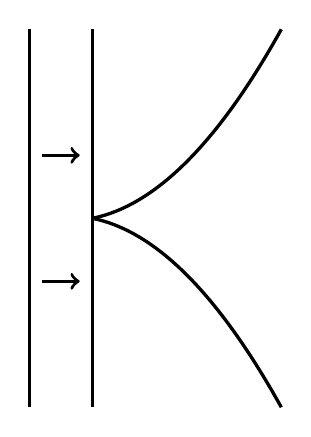
\begin{tikzpicture}[line width=1.2pt, scale=0.8] % 设置全局线条粗细

    % 1. 绘制左侧两条垂直的平行线（代表障碍物或狭缝）
    \draw (0, -3) -- (0, 3);
    \draw (1, -3) -- (1, 3);

    % 2. 绘制两个向右的入射箭头
    \draw[->] (0.2, 1) -- (0.8, 1);
    \draw[->] (0.2, -1) -- (0.8, -1);

    % 3. 绘制右侧向上和向下扩散的曲线（代表衍射波）
    % 使用贝塞尔曲线 (.. controls ..) 模拟平滑扩散的形状
    \draw (1, 0) .. controls (2, 0.2) and (3, 1.2) .. (4, 3);
    \draw (1, 0) .. controls (2, -0.2) and (3, -1.2) .. (4, -3);

\end{tikzpicture}
\end{center}
\end{aside}

\subsection*{射影平面曲线}

$k$ 上的射影平面是
\[
\mathbb{P}^2(k) = \{(x,y,z)\in k^3 \mid (x,y,z)\neq(0,0,0)\}/{\sim},
\]
其中 $(x,y,z)\sim(x',y',z')$ 当且仅当存在 $c\neq 0\in k$ 使 $(x',y',z') = (cx,cy,cz)$. 记 $(x:y:z)$ 为 $(x,y,z)$ 的等价类——冒号意在提示只有比值有意义. 设 $P\in\mathbb{P}^2(k)$, 表示 $P$ 的三元组 $(x,y,z)$ 落在 $k^3$ 中过原点的一条直线 $L(P)$ 上, 且 $P\mapsto L(P)$ 是 $\mathbb{P}^2(k)$ 到所有此类直线集合的双射. 射影 $n$-空间 $\mathbb{P}^n(k)$ 可类似定义.

设 $U_2(k) = \{(x:y:z) \mid z\neq 0\}$, $L_\infty(k) = \{(x:y:z) \mid z = 0\}$. 则
\[
(x,y)\mapsto(x:y:1)\colon\mathbb{A}^2(k)\to U_2(k), \qquad
(x,y)\mapsto(x:y:0)\colon\mathbb{P}^1(k)\to L_\infty(k)
\]
都是双射. 且 $\mathbb{P}^2(k)$ 是 ``仿射平面'' $U_2$ 与 ``无穷远直线'' $L_\infty$ 的无交并:
\[
\mathbb{P}^2(k) = U_2(k)\sqcup L_\infty(k).
\]
直线 $aX + bY + cZ = 0$ ($a,b$ 不全为零) 与 $L_\infty$ 交于点 $(-b:a:0)$, 它只依赖仿射直线 $aX + bY + c = 0$ 的斜率. 可以把 $\mathbb{P}^2$ 想象为仿射平面 $U_2$ 对每一族平行线恰好添上一个点.

一个非常数的齐次多项式 $F\in k[X,Y,Z]$, 假定其在 $k^{\mathrm{al}}$ 中无重复因子, 定义了 $k$ 上的一条射影平面曲线 (projective plane curve)\index{sheyingpingmianquxian@射影平面曲线(projective plane curve)} $C_F$, 它在任一包含 $k$ 的域 $K$ 中的点集为 $F$ 在 $\mathbb{P}^2(K)$ 中的零点:
\[
C_F(K) = \{(x:y:z)\in\mathbb{P}^2(K) \mid F(x,y,z) = 0\}.
\]
注意, 因 $F$ 齐次,
\[
F(cx,cy,cz) = c^{\deg F}F(x,y,z), \qquad c\in k^{\times},
\]
故虽然谈论 $F$ 在 $\mathbb{P}^2$ 的某点 $P$ 处的值无意义, 但谈论 $F$ 在 $P$ 处是否为零是有意义的. 同样, 我们不区分曲线 $C_F$ 与 $C_{cF}$ ($c\in k^{\times}$). 一条平面射影曲线 (唯一地) 是一些不可约射影平面曲线 (由不可约多项式定义的那些) 的并. $F$ 的次数称为曲线 $C_F$ 的次数 (degree).\index{quxiandecishu@曲线的次数(degree of a curve)}

\begin{example} \label{thm:1.1.15} 
曲线
\[
Y^2Z = X^3 + aXZ^2 + bZ^3
\]
与无穷远直线交于点 $(0:1:0)$, 即与所有竖直线相同的一点. 这在几何上是合理的, 因为当 $x\to\infty$ 时, 实仿射曲线 $Y^2 = X^3 + aX + b$ 的切线的斜率趋于无穷 (见前言 p.~\pageref{chapter:intro} 的图).
\end{example}

设 $U_1(k) = \{(x:y:z) \mid y\neq 0\}$, $U_0(k) = \{(x:y:z) \mid x\neq 0\}$. 则 $U_1$ 与 $U_0$ 也以自然方式成为仿射平面:
\[
(x,z)\longleftrightarrow(x:1:z)\colon\mathbb{A}^2(k)\cong U_1(k), \qquad
(y,z)\longleftrightarrow(1:y:z)\colon\mathbb{A}^2(k)\cong U_0(k).
\]
因 $x,y,z$ 至少有一个非零,
\[
\mathbb{P}^2 = U_0\cup U_1\cup U_2.
\]
射影平面曲线 $C = C_F$ 是三条仿射平面曲线的并:
\[
C = C_0\cup C_1\cup C_2, \qquad C_i = C\cap U_i.
\]
{\emergencystretch=3em 把每个 $U_i$ 以自然方式等同于 $\mathbb{A}^2$ 时, $C_0, C_1, C_2$ 分别等同于由多项式 $F(1,Y,Z)$, $F(X,1,Z)$, $F(X,Y,1)$ 定义的仿射曲线.\par}

\begin{example} \label{thm:1.1.16} 
曲线
\[
C\colon Y^2Z = X^3 + aXZ^2 + bZ^3
\]
由两条仿射曲线覆盖, 即
\[
C_2\colon Y^2 = X^3 + aX + b \qquad \text{与} \qquad C_1\colon Z = X^3 + aXZ^2 + bZ^3.
\]
\end{example}

切线、重数、相交数等概念可通过下述方式搬到射影曲线上: 射影曲线 $C$ 的每个点 $P$ 至少位于某个仿射曲线 $C_i$ 上. 若 $P\in C(k)$ 作为某仿射曲线 $C_i$ 的点是非奇异的, 则在所有包含 $P$ 的 $C_i$ 中都非奇异. 其他概念也有类似的结论.

\begin{exercise} \label{thm:1.1.17} 
设 $P$ 是射影平面曲线 $C = C_F$ 上的点. 证明 $P$ 奇异当且仅当
\[
\Bigl(\frac{\partial F}{\partial X}\Bigr)_P = \Bigl(\frac{\partial F}{\partial Y}\Bigr)_P = \Bigl(\frac{\partial F}{\partial Z}\Bigr)_P = 0.
\]
当 $P$ 非奇异时, 证明射影直线
\[
L\colon \Bigl(\frac{\partial F}{\partial X}\Bigr)_P X + \Bigl(\frac{\partial F}{\partial Y}\Bigr)_P Y + \Bigl(\frac{\partial F}{\partial Z}\Bigr)_P Z = 0
\]
具有性质: 对每个满足 $P\in U_i$ 的 $i$, $L\cap U_i$ 是仿射曲线 $C_i$ 在 $P$ 处的切线.
\end{exercise}

\subsection*{Bezout 定理}\index{Bezout@Bezout 定理(Bezout's theorem)}

\begin{theorem}[Bezout] \label{thm:1.1.18} 
设 $C$ 与 $D$ 为 $k$ 上次数分别为 $m$ 与 $n$ 的射影平面曲线, 且无公共分支. 则 $C$ 与 $D$ 在 $k^{\mathrm{al}}$ 上恰好相交于计入重数的 $mn$ 个点, 即
\[
\sum_{P\in C(k^{\mathrm{al}})\cap D(k^{\mathrm{al}})} I(P, C\cap D) = mn.
\]
\end{theorem}

\begin{proof}
初等证明见 \cite[\S5.3]{fulton1969}.
\end{proof}

设 $C$ 与 $D$ 为 $k$ 上次数分别为 $m$ 与 $n$ 的射影平面曲线. 若 $C(k^{\mathrm{al}})\cap D(k^{\mathrm{al}})$ 中恰有 $mn$ 个点, 则 Bezout 定理与 \ref{thm:1.1.13} 表明这些点在 $C$ 与 $D$ 上都非奇异; 若点多于 $mn$ 个, 则曲线必有公共分支.

\begin{aside} \label{thm:1.1.19} 
在 $\mathbb{C}$ 上, 映射
\[
(F,G) \mapsto \sum_{P\in C_F(\mathbb{C})\cap C_G(\mathbb{C})} I(P, C_F\cap C_G)
\]
关于 $F$ 与 $G$ 的系数 (对 $\mathbb{N}$ 的离散拓扑) 连续. 因此总相交数在齐次多项式的连续族上恒定, 这使得在证明 Bezout 定理时可取 $F = X^m$, $G = Y^n$. 则 $P = (0:0:0)$ 是两条曲线上唯一的公共点, 且
\[
I(P, C_{X^m}\cap C_{Y^n}) = I(X^m, Y^n) = mn,
\]
即证得定理. 类似论证对任意域都成立, 只要先证明总相交数在代数族上恒定 (cf.\ \cite[III, 2.2]{shafarevich1994}).
\end{aside}

\begin{example} \label{thm:1.1.20} 
由 Bezout 定理, 一条 $m$ 次曲线与无穷远直线计入重数地恰好交于 $m$ 个点. 我们钟爱的曲线
\[
C\colon Y^2Z = X^3 + aXZ^2 + bZ^3
\]
与 $L_\infty$ 交于唯一点 $P = (0:1:0)$, 但 (见~\ref{thm:1.1.8})
\[
I(P, L_\infty\cap C) = I(Z, Z - X^3 - aXZ - bZ^3) = I(Z, X^3) = 3.
\]
一般地, 曲线 $C$ 上的非奇异点 $P$ 若其切线与 $C$ 在 $P$ 处的相交重数 $\ge 3$, 则称为拐点 (point of inflection, 或 flex).\index{guaidian@拐点(point of inflection)}\footnote{有时还要求相交重数为奇数.} 若相交重数等于 $3$, 则称拐点为普通的 (ordinary).\index{guaidian@拐点(point of inflection)!putong@普通(ordinary)} 三次曲线上的拐点总是普通的.
\end{example}

\begin{remark} \label{thm:1.1.21} 
由 Bezout 定理, 射影平面曲线的任意两个不可约分支都有公共点 (可能在 $k$ 的某个有限扩张中), 该点由~\ref{thm:1.1.4}b 是奇异的. 因此, 非奇异射影平面曲线几何不可约.
\end{remark}

\subsection*{附录：结式}

设 $f(X) = s_0X^m + s_1X^{m-1} + \cdots + s_m$ 与 $g(X) = t_0X^n + t_1X^{n-1} + \cdots + t_n$ 为系数在 $k$ 中的多项式. $f$ 与 $g$ 的结式 (resultant)\index{jieshi@结式(resultant)} $\operatorname{Res}(f,g)$ 定义为行列式
\[
\begin{vmatrix}
s_0 & s_1 & \cdots & s_m & & \\
& s_0 & \cdots & s_{m-1} & s_m & \\
& & \ddots & & & \\
& & & s_0 & s_1 & \cdots & s_m\\
t_0 & t_1 & \cdots & t_n & & \\
& t_0 & \cdots & t_{n-1} & t_n & \\
& & \ddots & & & \\
& & & t_0 & t_1 & \cdots & t_n
\end{vmatrix}
\]
其中有 $n$ 行 $s_i$ 与 $m$ 行 $t_j$, 故矩阵为 $(m+n)\times(m+n)$; 所有空白处填零. 结式是 $f$ 与 $g$ 的系数的多项式.

\begin{proposition} \label{thm:1.1.22} 
结式 $\operatorname{Res}(f,g) = 0$ 当且仅当
\begin{enumerate}[label=\textup{(\alph*)}]
\item $s_0$ 与 $t_0$ 都为零; 或
\item 两多项式在 $k^{\mathrm{al}}$ 中有公共根.\footnote{校对注：原书把公共根写为在 $k$ 中. 对一般域，这应是在 $k^{\mathrm{al}}$ 中；例如在 $k=\mathbb{R}$ 时，$f=g=X^2+1$ 的结式为零，却没有实根. 下文相应地在代数闭包上作根的分解，并将最大公因子的域扩张不变性陈述为非常数公共因子的存在性不变.}
\end{enumerate}
\end{proposition}

\begin{proof}
若 (a) 成立, 则行列式第一列为零, 故 $\operatorname{Res}(f,g) = 0$. 设 $a$ 为 $f$ 与 $g$ 的公共根, 则存在次数分别为 $m-1$ 与 $n-1$ 的多项式 $f_1, g_1\in k^{\mathrm{al}}[X]$ 使
\[
f(X) = (X-a)f_1(X), \qquad g(X) = (X-a)g_1(X).
\]
由这些等式得
\begin{equation} \label{eq:2}
f(X)g_1(X) - g(X)f_1(X) = 0.
\tag{2}
\end{equation}
把 \eqref{eq:2} 中 $X^{m+n-1},\dots,X,1$ 的系数置零, 我们发现 $f_1$ 与 $g_1$ 的系数是 $m+n$ 个未知数、$m+n$ 个线性方程组的解. 方程组的系数矩阵是矩阵 \eqref{eq:3} 的转置:
\begin{equation} \label{eq:3}
\begin{pmatrix}
s_0 & s_1 & \cdots & s_m & & & & \\
& s_0 & \cdots & s_{m-1} & s_m & & & \\
& & \ddots & & & & & \\
& & & s_0 & s_1 & \cdots & s_m & \\
t_0 & t_1 & \cdots & t_n & & & & \\
& t_0 & \cdots & t_{n-1} & t_n & & & \\
& & \ddots & & & & & \\
& & & t_0 & t_1 & \cdots & t_n
\end{pmatrix}
\tag{3}
\end{equation}
解的存在表明该矩阵行列式为零, 由此推出 $\operatorname{Res}(f,g) = 0$.

反之, 设 $\operatorname{Res}(f,g) = 0$ 但 $s_0$ 与 $t_0$ 均非零. 因上述矩阵行列式为零, 可解线性方程找到满足 \eqref{eq:2} 的多项式 $f_1, g_1$. $f$ 的根 $a$ 必也是 $f_1$ 或 $g$ 的根. 若是前者, 从 \eqref{eq:2} 左边消去 $X-a$, 考虑 $f_1/(X-a)$ 的根. 因 $\deg f_1 < \deg f$, 此论证最终导致 $f$ 的一个不是 $f_1$ 的根的根, 故它必是 $g$ 的根.
\end{proof}

注意, $k[X]$ 中多项式 $f,g$ 在 $k[X]$ 中有非常数公共因子当且仅当它们在 $k^{\mathrm{al}}[X]$ 中有非常数公共因子, 因为 Euclid 算法表明两个多项式的最大公因子在域扩张下不变 (\cite[2.10]{milne-ft}).

\begin{example} \label{thm:1.1.23} 
对 $m$ 次首一多项式 $f(X)$, $\operatorname{Res}(f, f') = (-1)^{m(m-1)/2}\operatorname{disc}(f)$. 设 $c_1,\dots,c_{m+n}$ 为矩阵 \eqref{eq:3} 的列. 则
\[
\begin{pmatrix}X^{n-1}f(X)\\ X^{n-2}f\\ \vdots\\ f(X)\\ X^{m-1}g(X)\\ \vdots\\ g(X)\end{pmatrix}
= X^{m+n-1}c_1 + \cdots + 1\cdot c_{m+n},
\]
\footnote{校对注：矩阵 \eqref{eq:3} 有 $n$ 行 $f$ 的系数与 $m$ 行 $g$ 的系数，因此左侧的幂次分别从 $n-1$ 与 $m-1$ 开始；原书在此处把两者互换. 原书随后还混用了 $c_0$ 与 $c_1$，此处统一采用前面定义的 $c_1,\dots,c_{m+n}$.} 故 $\operatorname{Res}(f,g) \overset{\text{def}}{=} \det(c_1,\dots,c_{m+n}) = \det(c_1,\dots,c_{m+n-1}, c)$, 其中 $c$ 是上式左边的向量. 展开最后一个行列式, 得
\[
\operatorname{Res}(f,g) = a(X)f(X) + b(X)g(X),
\]
其中 $a(X)$ 与 $b(X)$ 分别是次数 $\le n-1$ 与 $\le m-1$ 的多项式. 若 $f(X)$ 与 $g(X)$ 的系数在整环 $R$ (例如 $\mathbb{Z}$ 或 $k[Y]$) 中, 则 $\operatorname{Res}(f,g)\in R$, 且多项式 $a(X)$, $b(X)$ 的系数也在 $R$ 中.
\end{example}

\begin{proposition} \label{thm:1.1.24} 
设 $f(X,Y), g(X,Y)\in k[X,Y]$, 且 $r(X)\in k[X]$ 为把 $f, g$ 视为系数在 $k[X]$ 中、关于 $Y$ 的多项式时的结式.
\begin{enumerate}[label=\textup{(\alph*)}]
\item 存在 $a(X,Y), b(X,Y)\in k[X,Y]$ 使
\[
af + bg = r(X)\in k[X]
\]
且 $\deg_Y(a) < \deg_Y(g)$, $\deg_Y(b) < \deg_Y(f)$.
\item 多项式 $r = 0$ 当且仅当 $f$ 与 $g$ 在 $k[X,Y]$ 中有关于 $Y$ 的次数为正的公共因子.\footnote{校对注：原书未限制公共因子关于 $Y$ 的次数. 例如 $f=X$、$g=X(Y+1)$ 有公共因子 $X$，但关于 $Y$ 的结式为 $X$，不为零. 这里的判据来自 $k(X)[Y]$ 中的公共因子，故须排除仅依赖 $X$ 的因子.}
\end{enumerate}
\end{proposition}

\begin{proof}
\begin{enumerate}[label=\textup{(\alph*)}]
\item 由上面的讨论直接得到.
\item 我们知道 $r = 0$ 当且仅当 $f$ 与 $g$ 在 $k(X)[Y]$ 中有公共因子, 但由 Gauss 引理 (\cite[4.5]{milne-ca}), 这等价于它们在 $k[X,Y]$ 中有关于 $Y$ 的次数为正的公共因子.
\end{enumerate}
\end{proof}

\begin{corollary} \label{thm:1.1.25} 
若多项式 $f$ 与 $g$ 在 $k[X,Y]$ 中无公共因子, 则对任意包含 $k$ 的域 $K$, 它们在 $K[X,Y]$ 中无公共因子.
\end{corollary}

\begin{proof}
因 $f$ 与 $g$ 的结式无论我们在 $k$ 上还是在 $K$ 上工作都相同, 这由命题的 (b) 推出.
\end{proof}

\paragraph{齐次多项式的结式}
齐次多项式
\[
F(X,Y) = s_0X^m + s_1X^{m-1}Y + \cdots + s_mY^m, \qquad
G(X,Y) = t_0X^n + t_1X^{n-1}Y + \cdots + t_nY^n
\]
的结式按非齐次情形定义.

\begin{proposition} \label{thm:1.1.26} 
结式 $\operatorname{Res}(F,G) = 0$ 当且仅当 $F$ 与 $G$ 在 $\mathbb{P}^1(k^{\mathrm{al}})$ 中有非平凡零点.
\end{proposition}

\begin{proof}
$F(X,Y)$ 在 $\mathbb{P}^1(k^{\mathrm{al}})$ 中的非平凡零点形如 (a) $(a:1)$, 其中 $a$ 是 $F(X,1)$ 的根; 或 (b) $(1:0)$, 当 $s_0 = 0$ 时. 由于对 $G(X,Y)$ 有类似结论, 本命题是命题 \ref{thm:1.1.22} 的重述.
\end{proof}

计算机代数程序可以计算结式. 例如, 在 Pari/gp 中输入
\begin{verbatim}
polresultant((x+a)^5,(x+b)^5,x)
\end{verbatim}
给出的答案是 $(b-a)^{25}$, 意思是两多项式有公共根当且仅当 $a = b$, 而这可能以 $25$ 种方式发生.

\begin{aside} \label{thm:1.1.27} 
最后一个命题有几何解释. 取 $k$ 代数闭, 把 $F$ 与 $G$ 的系数视为未定元. 设 $V$ 为 $\mathbb{A}^{m+n+2}\times\mathbb{P}^1$ 中 $F(s_0,\dots,s_m;X,Y)$ 与 $G(t_0,\dots,t_n;X,Y)$ 都为零的子集. 命题说 $V$ 在 $\mathbb{A}^{m+n+2}$ 上的投影是 $\operatorname{Res}(F,G)$ (视为 $s_i, t_i$ 的多项式) 为零的集合. 换言之, 命题告诉我们 Zariski 闭集 $V$ 的投影正是由 $F$ 与 $G$ 的结式定义的 Zariski 闭集.

{\emergencystretch=3em 消去理论 (elimination theory) 更一般地做这件事: 对在 $X_i$ 中齐次的多项式 $P_i(T_1,\dots,T_m;\allowbreak X_0,\dots,X_n)$, 它给出寻找多项式 $R_j(T_1,\dots,T_m)$ 的算法, 使 $P_i(a_1,\dots,a_m;\allowbreak X_0,\dots,X_n)$ 有公共零点当且仅当对所有 $j$ 有 $R_j(a_1,\dots,a_m) = 0$. 例如见 \cite[Chap. 8, \S5]{cox2007}.\par}
\end{aside}

\begin{remarkstar}
平面代数曲线的历史可追溯到 2000 多年前——见 \cite[第一章]{brieskorn1986}. Newton\index{Newton} 对实三次平面曲线作了首次系统研究, 把它们分成 72 类 (但漏掉 6 类).
\end{remarkstar}

\section{平面曲线上的有理点}\label{sec:1.2}

对 $\mathbb{Q}$ 上的射影平面曲线 $C_F$, 两个基本问题是:
\begin{enumerate}[label=\textup{(\alph*)}]
\item $C_F$ 是否有坐标在 $\mathbb{Q}$ 中的点, 即 $F(X,Y,Z)$ 是否在 $\mathbb{Q}$ 中有非平凡零点?
\item 若 (a) 的答案是肯定的, 能否描述点集?
\end{enumerate}
还可问是否存在回答这些问题的算法. 例如, 我们可能知道一条曲线只有有限个点, 却没有算法找到这些点或确定其数目.

本节给出该主题的概述. 为简单起见, 全文假设 $C = C_F$ 几何不可约, 即 $F(X,Y,Z)$ 在 $\mathbb{Q}[X,Y,Z]$ 中不可约且在 $\mathbb{Q}^{\mathrm{al}}$ 上仍不可约.

先作一个全书都很有用的观察. 设 $f(X,Y) = \sum a_{ij}X^iY^j$ 为系数 $a_{ij}$ 在域 $k$ 中的多项式, $K$ 为 $k$ 的 Galois 扩张 (可能无限). 若 $(a,b)\in K\times K$ 是 $f(X,Y)$ 的零点, 则对所有 $\sigma\in\operatorname{Gal}(K/k)$, $(\sigma a,\sigma b)$ 也是零点, 因为
\[
f(\sigma a,\sigma b) = \sum a_{ij}(\sigma a)^i(\sigma b)^j = \sigma\Bigl(\sum a_{ij}a^ib^j\Bigr) = \sigma f(a,b) = 0.
\]
因此 $\operatorname{Gal}(K/k)$ 作用在 $C_f(K)$ 上. 更一般地, 若 $C_1, C_2, \dots$ 是 $k$ 上的仿射平面曲线, 则 $\operatorname{Gal}(K/k)$ 稳定 $K\times K$ 的子集 $C_1(K)\cap C_2(K)\cap\cdots$. 把此结论应用于曲线
\[
f = 0, \qquad \frac{\partial f}{\partial X} = 0, \qquad \frac{\partial f}{\partial Y} = 0,
\]
我们看到 $\operatorname{Gal}(K/\mathbb{Q})$ 稳定 $C_f$ 的奇异点集. 对射影平面曲线有类似结论.

\subsection*{一次曲线}

此时曲线是直线
\[
C\colon aX + bY + cZ = 0, \qquad a,b,c\in\mathbb{Q}, \text{ 不全为零}.
\]
它总有坐标在 $\mathbb{Q}$ 中的点, 且可以参数化这些点——例如若 $c\neq 0$, 则映射
\[
(s:t)\mapsto(s:t:-\tfrac{a}{c}s - \tfrac{b}{c}t)
\]
对所有包含 $\mathbb{Q}$ 的域 $K$ 都是 $\mathbb{P}^1(K)$ 到 $C(K)$ 的双射.

\subsection*{二次曲线}

此时 $F(X,Y,Z)$ 是 3 个变量的二次型\index{ercixing@二次型(quadratic form)}, $C$ 是圆锥曲线 (conic). 注意 $C$ 不能奇异: 过重数 $m\ge 2$ 的点 $P$ 的非切线 $L$ 将与 $C$ 交于第二点 $Q$, 而总相交数
\[
I(P, L\cap C) + I(Q, L\cap C) \overset{\text{\ref{thm:1.1.13}}}{\ge} m + 1
\]
违反 Bezout 定理.

有时容易看出 $C(\mathbb{Q})$ 为空. 例如, $X^2 + Y^2 + Z^2$ 在 $\mathbb{Q}$ 中无非平凡零点, 因为它在 $\mathbb{R}$ 中无非平凡零点. 类似地, $X^2 + Y^2 - 3Z^2$ 无非平凡零点, 因为若有, 则它有零点 $(x,y,z)$ 满足 $x,y,z\in\mathbb{Z}$ 且 $\gcd(x,y,z) = 1$; $\mathbb{Z}/3\mathbb{Z}$ 中只有 $0$ 与 $1$ 是平方, 故
\[
x^2 + y^2 \equiv 0 \pmod{3} \implies x\equiv 0\equiv y \pmod{3};
\]
但此时 $3$ 整除 $z$, 与假设 $\gcd(x,y,z) = 1$ 矛盾.

1785 年, Legendre 表明此类论证可以变成判定 $C_F(\mathbb{Q})$ 是否非空的程序. 他先证明, 经初等变量替换, $F$ 可化为对角形式
\[
F = aX^2 + bY^2 + cZ^2, \qquad a,b,c\in\mathbb{Z}, \ a,b,c \text{ 无平方因子}.
\]
他再证明, 若 $abc\neq 0$ 且 $a,b,c$ 不全同号, 则 $F(X,Y,Z)$ 在 $\mathbb{Q}$ 中有非平凡零点当且仅当 $-bc$, $-ca$, $-ab$ 分别是模 $a$, $b$, $c$ 的平方. 由二次互反律\index{dingli@定理(theorem)!ercihufanlv@二次互反律(quadratic reciprocity law)} (IV\ref{thm:4.8.5}), 这蕴含: 存在以简单方式依赖于 $F$ 系数的整数 $m$, 使 $C_F(\mathbb{Q})\neq\varnothing$ 当且仅当 $F(X,Y,Z)\equiv 0\pmod{m}$ 有与 $m$ 互素的整数解. 见~\ref{thm:1.2.18}.

现在设 $C$ 有坐标在 $\mathbb{Q}$ 中的点 $P_0$. 能否描述所有点? $\mathbb{Q}$ 上的直线计入重数地总是与 $C$ 恰好交于两点 (Bezout 定理). 若两点重合, 则直线与 $C$ 相切. 否则, 点对在 $\operatorname{Gal}(\mathbb{Q}^{\mathrm{al}}/\mathbb{Q})$ 的作用下稳定, 故若其中一点系数在 $\mathbb{Q}$ 中, 则两点都在. $\mathbb{P}^2$ 中过 $P_0$ 的直线构成一个 ``$\mathbb{P}^1$'', 把过 $P_0$ 的直线送到其第二个交点, 是 $\mathbb{P}^1(\mathbb{Q})$ 到 $C(\mathbb{Q})$ 的双射. 例如, 取 $P_0$ 为曲线 $C\colon X^2 + Y^2 = Z^2$ 上的点 $(-1:0:1)$. 过 $P_0$、斜率为 $b/a$ ($a,b\in\mathbb{Q}$) 的直线 $bX - aY + bZ$ 与 $C$ 交于点 $(a^2-b^2 : 2ab : a^2+b^2)$. 这样, 我们得到 $C$ 上坐标在 $\mathbb{Q}$ 中的点的参数化 $(a:b)\mapsto(a^2-b^2:2ab:a^2+b^2)$.

\subsection*{三次曲线}

设 $C\colon F(X,Y,Z) = 0$ 为 $\mathbb{Q}$ 上次数 $3$ 的射影平面曲线. 若 $C$ 奇异, 则 Bezout 定理表明它只有一个奇异点, 且其重数为 $2$. 奇异点 $P_0$ 的坐标在 $\mathbb{Q}$ 的某个有限扩张 $K$ 中, 可取 $K$ 在 $\mathbb{Q}$ 上 Galois, 但 $\operatorname{Gal}(K/\mathbb{Q})$ 稳定 $C(K)$ 中的奇异点集, 故固定 $P_0$, 从而 $P_0\in C(\mathbb{Q})$. 此时过 $P_0$ 的直线与曲线恰好交于另一个点 (可能与 $P_0$ 重合), 故再次得到 $C$ 上坐标在 $\mathbb{Q}$ 中的点的参数化.

非奇异三次曲线将是本书其余部分的主题. 我们将看到 Legendre 的论证对非奇异三次曲线失败. 例如,
\[
3X^3 + 4Y^3 + 5Z^3
\]
有非平凡的实零点, 且对每个整数 $m$ 有非平凡模 $m$ 零点, 但它在 $\mathbb{Q}$ 中没有非平凡零点.

设 $C$ 为 $\mathbb{Q}$ 上的非奇异三次曲线. 由 Bezout 定理, 直线计入重数地与曲线交于三点. 若其中两点系数在 $\mathbb{Q}$ 中, 则第三点也系数在 $\mathbb{Q}$ 中.\footnote{把 $Y = aX + b$ 代入定义仿射三次曲线的多项式, 得到 $X$ 的系数在 $\mathbb{Q}$ 中的三次多项式, 其两个根在 $\mathbb{Q}$ 中; 于是第三个根也在 $\mathbb{Q}$ 中.} 因此, $C(\mathbb{Q})$ 中两点的弦与曲线交于 $C(\mathbb{Q})$ 中的第三点, 且 $C(\mathbb{Q})$ 中某点的切线与曲线交于 $C(\mathbb{Q})$ 中的另一点.

在一篇著名的论文 (1922 年发表) 中, Mordell\index{Mordell} 证明了以下定理.

\begin{theorem}[有限基定理] \label{thm:1.2.1}\index{dingli@定理(theorem)!youxianji@有限基定理(finite basis theorem)} 
设 $C$ 为 $\mathbb{Q}$ 上的非奇异三次曲线. 则存在 $C(\mathbb{Q})$ 中的有限点集, 使 $C(\mathbb{Q})$ 中其他每个点都能由这些点经反复的弦与切线构造而得到.
\end{theorem}

事实上, $C(\mathbb{Q})$ 若非空, 则有自然的交换群结构 (见下节), 而有限基定理说 $C(\mathbb{Q})$ 有限生成. 迄今仍无被证明的算法可求该群的秩.

\begin{remark} \label{thm:1.2.2} 
对 $\mathbb{Q}$ 上的奇异三次曲线 $C$, 非奇异点仍构成群, 可能同构于 $(\mathbb{Q},+)$ 或 $(\mathbb{Q}^{\times},\times)$ (见 II, \S\ref{sec:2.3}), 两者都不有限生成——$(\mathbb{Q},+)$ 的任何有限生成子群中元素有公共分母, 而 $(\mathbb{Q}^{\times},\times)$ 的有限生成子群只能含有限多个素数. 因此, 有限基定理对奇异三次曲线失败.
\end{remark}

\subsection*{亏格 $> 1$ 的曲线}

$\mathbb{Q}$ 上非奇异射影曲线 $C$ 的亏格 (genus)\index{kuige@亏格(genus)} 是 Riemann 曲面 $C(\mathbb{C})$ 的亏格. 更一般地, $\mathbb{Q}$ 上任意曲线的亏格是其函数域\index{hanshuyu@函数域(function field)}所对应的非奇异射影曲线的亏格 (\cite[\S7.5, Cor.\ to Theorem 3]{fulton1969}). Mordell 在 1922 年的论文中猜想, \cite{faltings1983} 证明了: 亏格 $> 1$ 的每条曲线都只有有限多个坐标在 $\mathbb{Q}$ 中的点. 这适用于次数至少为 $4$ 的每条非奇异射影平面曲线, 也适用于次数相对其奇点重数足够大的每条奇异射影平面曲线 (见本章后面的 \ref{thm:1.6.5}).

\begin{remark} \label{thm:1.2.3} 
设 $P\in\mathbb{P}^2(\mathbb{Q})$. 选取 $P$ 的代表元 $(a:b:c)$, 其中 $a,b,c$ 为无公因子的整数, 定义 $P$ 的高度 (height) $H(P) = \max(|a|,|b|,|c|)$. 对任意 $B > 0$, 只有有限多个 $P$ 满足 $H(P) < B$.

对亏格 $> 1$ 的曲线 $C$, 存在 $C(\mathbb{Q})$ 中点数的有效界, 但就定义 $C$ 的多项式而言, 对 $P\in C(\mathbb{Q})$ 的高度没有已知的有效界. 若有这样的界, 则通过有限搜索即可找到 $C(\mathbb{Q})$ 中的点. 见 \cite[F.4.2]{hindry2000} 对该问题的讨论.
\end{remark}

\begin{aside} \label{thm:1.2.4} 
对 Mordell 猜想有启发式解释. 设 $C$ 为 $\mathbb{Q}$ 上亏格 $g\ge 1$ 的曲线. 若 $C(\mathbb{Q})$ 非空, 则 $C$ 嵌入其 Jacobi 簇 $J$, 后者是维数 $g$、带群结构的射影簇, 即 阿贝尔簇. Weil\index{Weil} 推广的有限基定理说 $J(\mathbb{Q})$ 有限生成. 因此在 $g$ 维集合 $J(\mathbb{C})$ 中, 有可数集 $J(\mathbb{Q})$ 和 (看起来无关的) 一维集 $C(\mathbb{C})$. 若 $g > 1$, 第二个集合含第一个集合中多于有限多个元素将是非同寻常的巧合.
\end{aside}

为继续讨论, 我们需要 $p$-进数域.

\subsection*{$p$-进数简介}

设 $p$ 为素数. 非零有理数 $a$ 可唯一表示为 $a = p^r\frac{m}{n}$, 其中 $m, n, r$ 为整数且 $m, n$ 不被 $p$ 整除. 令 $|a|_p = \frac{1}{p^r}$, 且 $|0|_p = 0$. 称 $|a|_p$ 为 $a$ 的 $p$-进赋值. 它有如下性质:
\begin{enumerate}[label=\textup{(\alph*)}]
\item $|a|_p = 0$ 当且仅当 $a = 0$;
\item $|ab|_p = |a|_p|b|_p$;
\item $|a+b|_p\le\max\{|a|_p,|b|_p\}$ ($\le |a|_p + |b|_p$).
\end{enumerate}
这些论断蕴含
\[
d_p(a,b) \overset{\text{def}}{=} |a-b|_p
\]
是 $\mathbb{Q}$ 上的平移不变度量, 称为 $p$-进度量. 注意对此度量而言有理数 $a, b$ 接近意味着它们的差被 $p$ 的高次幂整除. $p$-进数域 $\mathbb{Q}_p$ 是 $\mathbb{Q}$ 关于此度量的完备化. 下面解释这是什么意思.

有理数序列 $a_1, a_2, a_3, \dots$ 关于 $p$-进度量是 Cauchy 序列\index{Cauchy-xulie@Cauchy 序列(Cauchy sequence)}, 若对每个实数 $\varepsilon > 0$, 存在自然数 $N(\varepsilon)$ 使当 $m, n > N(\varepsilon)$ 时有 $|a_m - a_n|_p < \varepsilon$. 序列 $a_1, a_2, a_3, \dots$ 收敛到 $a\in\mathbb{Q}$, 若对每个实数 $\varepsilon > 0$, 存在自然数 $N(\varepsilon)$ 使当 $n > N(\varepsilon)$ 时有 $|a_n - a|_p < \varepsilon$.

设 $R$ 为 $\mathbb{Q}$ 中关于 $p$-进度量的一切 Cauchy 序列的集合. 用显然的运算它成为环. $R$ 的元素称为零的 (null), 若它收敛到 $0$. 零序列的集合是 $R$ 的理想 $I$, 而 $\mathbb{Q}_p$ 定义为商环 $R/I$. 它是域.

若 $\alpha = (a_n)_{n\ge 1}$ 是 $\mathbb{Q}$ 中的 Cauchy 序列, 则由性质 (c), 序列 $|a_n|_p$ 对大 $n$ 变成常数, 设此常数值为 $|\alpha|_p$. 映射 $\alpha\mapsto|\alpha|_p\colon R\to\mathbb{Q}$ 穿过 $\mathbb{Q}_p$ 且具有上面列出的性质 (a), (b), (c). 因此 $\mathbb{Q}$ 上的 $p$-进度量延拓到 $\mathbb{Q}_p$.

\begin{theorem} \label{thm:1.2.5} 
\begin{enumerate}[label=\textup{(\alph*)}]
\item 域 $\mathbb{Q}_p$ 完备, 即 $\mathbb{Q}_p$ 中每个 Cauchy 序列收敛到 $\mathbb{Q}_p$ 中的极限.
\item 把 $a\in\mathbb{Q}$ 送到常数 Cauchy 序列 $a,a,a,\dots$ 的等价类的映射, 是像稠密的单射同态 $\mathbb{Q}\hookrightarrow\mathbb{Q}_p$.
\end{enumerate}
\end{theorem}

\begin{proof}
练习.
\end{proof}

$p$-进整数环 $\mathbb{Z}_p$ 定义为 $\mathbb{Z}$ 在 $\mathbb{Q}_p$ 中的闭包. 这正是满足 $|\alpha|_p\le 1$ 的 $\alpha\in\mathbb{Q}_p$ 的集合. 每个 $p$-进整数 $a$ 可由唯一的级数表示:
\[
a_0 + a_1p + \cdots + a_ip^i + \cdots, \qquad 0\le a_i\le p-1,
\]
即存在唯一的整数序列 $a_0, a_1, \dots$ ($0\le a_i\le p-1$) 使上述级数的部分和构成表示 $a$ 的 Cauchy 序列. $a_i$ (若存在) 满足同余式
\[
a_0\equiv a \pmod{p\mathbb{Z}}, \quad \dots, \quad a_i \equiv \frac{a - (a_0 + \cdots + a_{i-1}p^{i-1})}{p^i} \pmod{p\mathbb{Z}}, \ \dots
\]
这证明了唯一性, 而这些同余式可用于归纳地定义 $a_i$: 利用 $\mathbb{Z}$ 在 $\mathbb{Z}_p$ 中稠密, 可得
\[
\mathbb{Z}/p^m\mathbb{Z} \cong \mathbb{Z}_p/p^m\mathbb{Z}_p, \qquad \text{所有 } m\ge 1.
\]
取极限, 得同构
\[
\varprojlim \mathbb{Z}/p^m\mathbb{Z} \cong \varprojlim \mathbb{Z}_p/p^m\mathbb{Z}_p \cong \mathbb{Z}_p.
\]

\begin{remark} \label{thm:1.2.6} 
\begin{enumerate}[label=\textup{(\alph*)}]
\item 上面的构造若把 $|\cdot|_p$ 换成通常的绝对值, 得到的是 $\mathbb{R}$ 而非 $\mathbb{Q}_p$.
\item 正如实数可用小数表示, $p$-进数可表示为如下形式的无穷级数:
\[
a_{-n}p^{-n} + \cdots + a_0 + a_1p + \cdots + a_mp^m + \cdots, \qquad 0\le a_i\le p-1.
\]
这可通过 $\mathbb{Q}_p^{\times} = p^{\mathbb{Z}}\cdot\mathbb{Z}_p^{\times}$ (直积) 证明.
\end{enumerate}
$p$-进整数环 $\mathbb{Z}_p$ 紧致, 且它在 $\mathbb{Q}_p$ 中开. 因此 $\mathbb{Q}_p$ 局部紧致. $p$-进数与当前讨论的相关性由下一个论断解释.

设 $f(X_0,\dots,X_n)\in\mathbb{Z}[X_0,\dots,X_n]$ 为齐次型. 假设对每个自然数 $N$, 存在整数 $a_0^{(N)},\dots,a_n^{(N)}$, 不全被 $p$ 整除, 使
\begin{equation} \label{eq:4}
f(a_0^{(N)},\dots,a_n^{(N)}) \equiv 0 \pmod{p^N}.
\tag{4}
\end{equation}
因 $\mathbb{Z}_p^{n+1}$ 紧致, 集合 $\{(a_0^{(N)},\dots,a_n^{(N)}) \mid N\in\mathbb{N}\}$ 在 $\mathbb{Z}_p^{n+1}$ 中有极限点 $(\alpha_0,\dots,\alpha_n)$, 且容易看出
\begin{equation} \label{eq:5}
f(\alpha_0,\dots,\alpha_n) = 0.
\tag{5}
\end{equation}
反之, 设 $(\alpha_0,\dots,\alpha_n)\in\mathbb{Q}_p^{n+1}$ 满足 \eqref{eq:5} 且不全为零. 缩放后可设 $\max_i|\alpha_i|_p = 1$. 对每个 $N\in\mathbb{N}$, 选取整数 $a_0^{(N)},\dots,a_n^{(N)}$ 使对所有 $j$ 有 $|a_j^{(N)} - \alpha_j|\le p^{-N}$. 则 $(a_0^{(N)},\dots,a_n^{(N)})$ 满足 \eqref{eq:4}.
\end{remark}

\begin{notation} \label{thm:1.2.7}\index{padic@p-进赋值(p-adic valuation)}
对 $a\in\mathbb{Q}^{\times}$, 若 $a = p^r\frac{m}{n}$ 且 $m, n$ 不被 $p$ 整除, 则令 $\ord\nolimits_p(a) = r$; 且令 $\ord\nolimits_p(0) = \infty$. 关于 $\infty$ 采用显然的约定, 我们有
\begin{enumerate}[label=\textup{(\alph*)}]
\item $\ord\nolimits_p(a) = \infty$ 当且仅当 $a = 0$;
\item $\ord\nolimits_p(ab) = \ord\nolimits_p(a) + \ord\nolimits_p(b)$;
\item $\ord\nolimits_p(a+b)\ge\min\{\ord\nolimits_p(a),\ord\nolimits_p(b)\}$, 且除非 $\ord\nolimits_p(a) = \ord\nolimits_p(b)$ 否则严格大于.
\end{enumerate}
特别地, $\ord\nolimits_p$ 是同态 $\mathbb{Q}^{\times}\to\mathbb{Z}$. 该同态由连续性延拓到 $\mathbb{Q}_p^{\times}$.
\end{notation}

\begin{remarkstar}
关于 $p$-进数更从容的讲解, 例如见 \cite{koblitz1977} 的第一章. 据 Ostrowski 定理\index{Ostrowski@Ostrowski 定理(Ostrowski's theorem)}, $\mathbb{R}$ 与各 $p$-进域 $\mathbb{Q}_p$ 是 $\mathbb{Q}$ 关于非平凡赋值仅有的完备化.
\end{remarkstar}

\subsection*{二次曲线与三次曲线续}

显然, 曲线有坐标在 $\mathbb{Q}$ 中的点的必要条件是它在 $\mathbb{R}$ 与所有 $\mathbb{Q}_p$ 中有坐标在其中的点. 事实上, 我们上面已观察到 $X^2 + Y^2 + Z^2$ 在 $\mathbb{Q}$ 中无非平凡零点, 因为它在 $\mathbb{R}$ 中无非平凡实零点; 而我们对 $X^2 + Y^2 - 3Z^2$ 的论证表明它在 $3$-进数域 $\mathbb{Q}_3$ 中无非平凡零点. Legendre 定理的现代解释是: 对二次曲线, 该条件也是充分的.

\begin{theorem}[Legendre] \label{thm:1.2.8} 
系数在 $\mathbb{Q}$ 中的二次型 $F(X,Y,Z)$ 在 $\mathbb{Q}$ 中有非平凡零点, 当且仅当它在 $\mathbb{R}$ 与所有 $\mathbb{Q}_p$ 中有非平凡零点.
\end{theorem}

\begin{proof}
见 \cite[Chapter 3]{cassels1991} 或 \cite[Chapter IV]{serre1973}.
\end{proof}

见下面 \ref{thm:1.2.18} 关于此陈述与 Legendre 原始陈述的关系.

\begin{aside} \label{thm:1.2.9} 
定理 \ref{thm:1.2.8} 对任意变量个数的二次型成立 (Hasse\index{Hasse}--Minkowski 定理). 证明的很好的讲解见 \cite[Chap.~IV]{serre1973}. 关键情形是 $3$ 个与 $4$ 个变量 ($2$ 个变量容易, 对 $\ge 5$ 个变量用关于 $n$ 的归纳), 证明所需的关键结果是二次互反律 (IV\ref{thm:4.8.5}).

若对某类多项式 (或代数簇\index{daishucu@代数簇(algebraic variety)}) 已知: 它在 $\mathbb{Q}$ 中有零点当且仅当它在 $\mathbb{R}$ 与所有 $\mathbb{Q}_p$ 中有零点, 则称该类满足 Hasse 原理, 或局部--整体原理 (local-global principle).\index{Hasse@Hasse 原理(Hasse principle)}\index{jubuzhengtiliyuanli@局部--整体原理(local-global principle)}
\end{aside}

\subsection*{Hensel 引理}

\begin{lemma} \label{thm:1.2.10} 
设 $f(X_1,\dots,X_n)\in\mathbb{Z}[X_1,\dots,X_n]$, $a\in\mathbb{Z}^n$ 满足: 对某个 $m\ge 0$,
\[
f(a) \equiv 0 \pmod{p^{2m+1}},
\]
但对某个 $i$,
\[
\Bigl(\frac{\partial f}{\partial X_i}\Bigr)(a) \not\equiv 0 \pmod{p^{m+1}}.
\]
则存在 $b\in\mathbb{Z}^n$ 使
\[
b\equiv a \pmod{p^{m+1}} \qquad \text{且} \qquad f(b)\equiv 0 \pmod{p^{2m+2}}.
\]
\end{lemma}

\begin{proof}
考虑泰勒展开
\[
f(X_1,\dots,X_n) = f(a_1,\dots,a_n) + \sum_{i=1}^n\Bigl(\frac{\partial f}{\partial X_i}\Bigr)_a(X_i - a_i) + \text{次数 }\ge 2 \text{ 的项}.
\]
令 $b_i = a_i + h_ip^{m+1}$, $h_i\in\mathbb{Z}$. 则
\[
f(b_1,\dots,b_n) = f(a_1,\dots,a_n) + \sum_{i=1}^n\Bigl(\frac{\partial f}{\partial X_i}\Bigr)_a h_ip^{m+1} + \text{被 } p^{2m+2} \text{ 整除的项}.
\]
我们必须选取 $h_i$ 使
\[
f(a_1,\dots,a_n) + \sum_{i=1}^n\Bigl(\frac{\partial f}{\partial X_i}\Bigr)_a h_ip^{m+1}
\]
被 $p^{2m+2}$ 整除. 由假设, 存在 $k\le m$ 使 $p^k$ 整除所有的 $\bigl(\frac{\partial f}{\partial X_i}\bigr)_a$, 但 $p^{k+1}$ 不整除它们的全部. 任何满足下式的 $h_i$ 都可以:
\[
\frac{f(a_1,\dots,a_n)}{p^{k+m+1}} + \sum_{i=1}^n\frac{\bigl(\frac{\partial f}{\partial X_i}\bigr)_a}{p^k}h_i \equiv 0 \pmod{p}.
\]
\end{proof}

\begin{remark} \label{thm:1.2.11} 
若引理中 $a$ 满足条件 $f(a)\equiv 0\pmod{p^{2m+r}}$ 对某个 $r\ge 1$, 则证明中的构造给出 $b$ 使 $b\equiv a\pmod{p^{m+r}}$ 且 $f(b)\equiv 0\pmod{p^{2m+r+1}}$.
\end{remark}

\begin{theorem}[Hensel 引理] \label{thm:1.2.12}\index{yinli@引理(lemma)!Hensel@Hensel(Hensel)} 
在引理的假设下, 存在 $b\in\mathbb{Z}_p^n$ 使 $f(b) = 0$ 且 $b\equiv a\pmod{p^{m+1}}$.
\end{theorem}

\begin{proof}
{\emergencystretch=3em 对引理应用, 得到 $a_{2m+2}\in\mathbb{Z}^n$ 使 $a_{2m+2}\equiv a\pmod{p^{m+1}}$ 且 $f(a_{2m+2})\equiv 0\pmod{p^{2m+2}}$. 第一个同余蕴含\par}
\[
\Bigl(\frac{\partial f}{\partial X_i}\Bigr)(a_{2m+2}) \equiv \Bigl(\frac{\partial f}{\partial X_i}\Bigr)(a) \pmod{p^{m+1}},
\]
{\emergencystretch=3em 故对某个 $i$, $\bigl(\frac{\partial f}{\partial X_i}\bigr)(a_{2m+2})\not\equiv 0\pmod{p^{m+1}}$. 对引理后的注记应用, 得到 $a_{2m+3}\in\mathbb{Z}^n$ 使 $a_{2m+3}\equiv a_{2m+2}\pmod{p^{m+2}}$ 且 $f(a_{2m+3})\equiv 0\pmod{p^{2m+3}}$. 如此继续, 得到 $n$-元组 Cauchy 序列 $a, a_{2m+2},$
$a_{2m+3}, \dots$. 设 $b$ 为它在 $\mathbb{Z}_p^n$ 中的极限. 映射 $f\colon\mathbb{Z}^n\to\mathbb{Z}$ 关于 $p$-进拓扑连续, 故\par}
\[
f(b) = f\Bigl(\lim_r a_{2m+r}\Bigr) = \lim_r f(a_{2m+r}) = 0.
\]
\end{proof}

\begin{example} \label{thm:1.2.13} 
设 $f(X)\in\mathbb{Z}[X]$, $\bar{f}(X)\in\mathbb{F}_p[X]$ 为它的模 $p$ 约化. 设 $a\in\mathbb{Z}$ 使 $\bar{a}\in\mathbb{F}_p$ 是 $\bar{f}(X)$ 的单根. 则 $\frac{d\bar{f}}{dX}(\bar{a})\neq 0$, 故定理表明 $\bar{a}$ 提升为 $f(X)$ 在 $\mathbb{Z}_p$ 中的根.
\end{example}

\begin{example} \label{thm:1.2.14} 
设 $F(X,Y,Z)$ 为 $\mathbb{Z}[X,Y,Z]$ 中的齐次多项式, $(a:b:c)\in\mathbb{P}^2(\mathbb{F}_p)$ 为曲线 $C_F$ 在 $\mathbb{F}_p$ 上的非奇异点. 则如上例, $(a:b:c)$ 提升为曲线 $C_F$ 上坐标在 $\mathbb{Z}_p$ 中的点.
\end{example}

\begin{example} \label{thm:1.2.15} 
设 $f(X,Y,Z)$ 为系数在 $\mathbb{Z}$ 中、判别式 $D\neq 0$ 的二次型. 若 $p\nmid D$, 则 $\bar{f}(X,Y,Z)$ 是 $\mathbb{F}_p$ 上判别式非零的二次型, 已知这样的型在 $\mathbb{F}_p$ 中有非平凡零点 (\cite[I, \S2]{serre1973}). 因此 $f(X,Y,Z)$ 在 $\mathbb{Q}_p$ 中有非平凡零点. 若 $p\mid D$, 则 Hensel 引理表明 $f(X,Y,Z)$ 若有``近似''零点, 则在 $\mathbb{Q}_p$ 中有非平凡零点.
\end{example}

\begin{exercise} \label{thm:1.2.16} 
设
\[
F(X,Y,Z) = 5X^2 + 3Y^2 + 8Z^2 + 6(YZ + ZX + XY).
\]
求 $(a,b,c)\in\mathbb{Z}^3$, 不全被 $13$ 整除, 使
\[
F(a,b,c)\equiv 0 \pmod{13^2}.
\]
\end{exercise}

\begin{exercise} \label{thm:1.2.17} 
考虑仿射平面曲线 $C\colon Y^2 = X^3 + p$. 证明约化曲线 $\bar{C}$ 在 $\mathbb{F}_p$ 上的点 $(0,0)$ 不能提升为 $C$ 上坐标在 $\mathbb{Z}_p^2$ 中的点. 这为什么不违反 Hensel 引理?
\end{exercise}

\begin{aside} \label{thm:1.2.18} 
设 $f(X,Y,Z)$ 为系数在 $\mathbb{Q}$ 中、判别式非零的二次型. 经初等变量替换, 可设 $f = aX^2 + bY^2 + cZ^2$ 且 $a,b,c$ 为无平方因子的整数. 若 $a, b, c$ 有公共素因子 $p$, 则用 $p^{-1}f$ 替换 $f$. 若两个系数 (譬如 $a$ 与 $b$) 有公共素因子 $p$, 则把 $Z$ 换成 $pZ$ 再除以 $p$. 因此, 在研究 $f = 0$ 的解时, 可设
\[
f(X,Y,Z) = aX^2 + bY^2 + cZ^2, \qquad a,b,c\in\mathbb{Z}, \ abc \text{ 无平方因子}.
\]
回忆 Legendre 证明 $f = 0$ 有非零解当且仅当
\begin{enumerate}[label=\textup{(\alph*)}]
\item $a,b,c$ 不全同号, 且
\item $-bc$, $-ca$, $-ab$ 分别是模 $a$, $b$, $c$ 的平方.
\end{enumerate}
我们证明条件 (a), (b) 的必要性. 设 $f = 0$ 有非零解 $(x,y,z)\in\mathbb{Q}^3$. 则当然 (a) 成立. 可设 $x,y,z\in\mathbb{Z}$ 且两两互素. 若 $x$ 与 $c$ 有公共素因子 $p$, 则 $p$ 整除 $y$, 与假设矛盾. 因此 $x$ 模 $c$ 可逆, 由 $ax^2 + by^2 + cz^2 = 0$ 推出 $-ab = (byx^{-1})^2$ 模 $c$. 类似地, $-bc$ 与 $-ca$ 分别是模 $a$ 与 $b$ 的平方.

我们证明 Legendre 原始定理蕴含定理 \ref{thm:1.2.9}: 若 $f$ 在 $\mathbb{R}$ 与对所有整除 $abc$ 的 $p$ 在 $\mathbb{Q}_p$ 中有非平凡零点, 则 Legendre 条件 (a), (b) 成立. 当然 (a) 成立. 设 $c = \prod_i p_i^{r_i}$. 因 $f$ 在 $\mathbb{Q}_{p_i}$ 中有非平凡零点, 上段论证表明 $-ab$ 是 $\mathbb{Z}_{p_i}/c\mathbb{Z}_{p_i} = \mathbb{Z}_{p_i}/p_i^{r_i}\mathbb{Z}_{p_i}$ 中的平方. 由于
\[
\mathbb{Z}/c\mathbb{Z} \cong \prod_i \mathbb{Z}/p_i^{r_i}\mathbb{Z} \qquad \text{(中国剩余定理)} \cong \prod_i \mathbb{Z}_{p_i}/p_i^{r_i}\mathbb{Z}_{p_i},
\]
推出 $-ab$ 是 $\mathbb{Z}/c\mathbb{Z}$ 中的平方. 类似地, $-bc$ 与 $-ca$ 分别是模 $a$ 与 $b$ 的平方.

定理 \ref{thm:1.2.9} 蕴含 Legendre 原始定理的证明同样初等, 只稍微长一点 (\cite{liu2019}).
\end{aside}

\begin{remarkstar}
用于构造新有理点的切线法可追溯到丢番图 (Diophantus\index{Diophantus}, 约公元 250 年), 且``深受费马喜爱''; 弦法为 Newton 所知. Hilbert\index{Hilbert} 与 Hurwitz\index{Hurwitz} 在 1890 年证明: 亏格零的曲线若有一个有理点, 则有无限多个, 全部由参数的整数值给出. 1901 年, Poincar\'e 发表了一篇关于曲线上有理点的长文, 试图把该主题从仅仅是关于单个方程的临时结果的集合中拯救出来. 虽然他通常被归功于猜想了有限基定理, 但他实际上是简单地假设了它. Beppo Levi 是第一个明确询问有限基定理是否成立的人. 在他非凡的 1922 年论文中, Mordell 证明了有限基定理, 并以相当随意的态度猜想 $\mathbb{Q}$ 上所有亏格 $> 1$ 的曲线都只有有限多个有理点 (Mordell 猜想). 两者都极其重要: 前者是丢番图几何的第一个一般定理, 后者是该主题最重要的未解决猜想之一, 直到 1983 年被 Faltings\index{Faltings} 证明.

关于这些主题的更多历史, 见 \cite{cassels1986}, \cite{schappacher1990} 与 \cite{schappacher1996}, 上述注释大部分取材于此.
\end{remarkstar}

\section{三次平面曲线上的群结构}\label{sec:1.3}

设 $C$ 为域 $k$ (为简单起见取为完美域) 上次数 $3$ 的非奇异射影平面曲线. 假设 $C(k)$ 非空, 选取点 $O\in C(k)$. 本节给出 $C(k)$ 上以 $O$ 为零元的群结构的几何构造.

由 Bezout 定理, 直线计入重数地与曲线交于三点. 给定 $P,Q\in C(k)$ (两者都不在对方处的切线上), 记 $PQ$ 为过 $P$ 与 $Q$ 的直线与 $C$ 的第三个交点. 给定 $P\in C(k)$, 记 $PP$ 为 $C$ 在 $P$ 处的切线与 $C$ 的第二个交点. 点 $PQ$ 与 $PP$ 的坐标在 $k$ 中.\footnote{当然, 存在 $k$ 的有限 Galois 扩张 $K$ 使 $PQ\in C(K)$, 但此时 $\operatorname{Gal}(K/k)$ 作用在集合 $\{P,Q,PQ\}$ 上, 故固定 $PQ$. 类似地 $PP\in C(k)$.} 注意 $PP = P$ 当且仅当 $P$ 是拐点.

对一对点 $P,Q\in C(k)$, 定义
\[
P + Q = O(PQ),
\]
即先画过 $P$ 与 $Q$ 的直线得到 $PQ$, 再画过 $O$ 与 $PQ$ 的直线得到 $P+Q$, 如下图所示:

\begin{center}
\begin{tikzpicture}[scale=1, thick]
    % 绘制椭圆曲线（上半支与下半支对称）
    \draw[thick] plot[smooth, tension=0.7] coordinates {
        (5, 3.2) (3.5, 1.4) (1.2, 0.6) (0, 0.4) (-0.5, 0) (0, -0.4) (1.2, -0.6) (3.
5, -1.8) (5, -3.2)
    };

    % 定义点坐标
    \coordinate (P) at (-0.5, -0.18);
    \coordinate (Q) at (0.9, 0.58);
    \coordinate (PQ) at (3.8, 1.76);
    \coordinate (PplusQ) at (3.8, -2.15);

    % 绘制割线（穿过 P, Q, PQ）
    \draw[thick] ($(P)!-0.3!(PQ)$) -- ($(P)!1.2!(PQ)$);

    % 绘制垂直线（穿过 PQ 和 P+Q）
    \draw[thick] (3.8, 2.3) -- (3.8, -2.7);

    % 标注各个点
    \node[above left] at (P) {$P$};
    \node[above] at (Q) {$Q$};
    \node[above left] at (PQ) {$PQ$};
    \node[left] at (PplusQ) {$P+Q$};
\end{tikzpicture}
\end{center}

\begin{theorem} \label{thm:1.3.1} 
上述构造使 $C(k)$ 成为交换群.
\end{theorem}

首先注意定义不依赖 $P,Q$ 的次序, 故
\[
P + Q = Q + P.
\]
其次注意
\[
O + P \overset{\text{def}}{=} O(OP) = P,
\]
故 $O$ 是中性元.

给定 $P\in C(k)$, 令 $P' = P(OO)$. 则 $PP' = OO$, 且 $O(PP') = O(OO) = O$, 即 $P + P' = O$.

\begin{center}
\begin{tikzpicture}[>=stealth, scale=1]
    % 1. 定义直线
    % 倾斜直线
    \draw[thick] (-0.5, 1.2) -- (4, 2.8) coordinate (L1_end);
    % 垂直直线
    \draw[thick] (3.3, 0) -- (3.3, 3) coordinate (L2_top);

    % 2. 定义交点和标记点
    % 手动指定 P 和 P' 的位置，使其看起来均匀
    \coordinate (P) at (0.3, 1.52);
    \coordinate (P_prime) at (2.0, 2.1);
    
    % 3. 绘制刻度线 (Ticks)
    % 角度大约是 19.6 度 (atan(1.6/4.5))，刻度线垂直于此
    \def\tickangle{109.6} 
    \draw[thick] ($(P) + (\tickangle:0.15)$) -- ($(P) + (\tickangle-180:0.15)$);
    \draw[thick] ($(P_prime) + (\tickangle:0.15)$) -- ($(P_prime) + (\tickangle-180:0.15)$);

    % 4. 绘制圆弧 (修正：凸面朝右)
    % 设定圆心在垂直线左侧，例如在 (2.0, 0.8) 处，半径 1.3
    % 这样圆弧会经过垂直线 (3.3, 0.8) 附近
    \draw[thick] (2.0, 0.8) ++(-35:1.3) arc (-35:35:1.3);

    % 5. 添加标签
    % P 和 P' 在上方
    \node[above=3pt, xshift=-2pt] at (P) {$P$};
    \node[above=3pt, xshift=-2pt] at (P_prime) {$P'$};
    
    % 右上角的两个 O
    \node[anchor=north west, inner sep=1pt] at (3.3, 2.5) {$OO$};
    
    % 圆弧交点处的 O
    \node[anchor=west] at (3.3, 0.8) {$O$};

\end{tikzpicture}
\end{center}

因此加法交换、有零元、且每个元素都有负元. 剩下需验证结合律, 即
\[
(P+Q) + R = P + (Q+R), \qquad \forall\, P,Q,R\in C(k).
\]
在第 \ref{sec:1.4} 节中, 我们将说明如何从 Riemann--Roch 定理推出它; 但这里我们概述一个优雅的几何证明.

\subsection*{结合律的几何证明}

在证明结合律时, 可以用更大的域替换 $k$, 故可设 $k$ 代数闭.

\begin{proposition} \label{thm:1.3.2} 
若 $\mathbb{P}^2$ 中两条三次曲线恰好交于九个点, 则经过其中八个点的每条三次曲线也经过第九个点.
\end{proposition}

\begin{proof}
三次型
\[
F(X,Y,Z) = a_1X^3 + a_2X^2Y + \cdots + a_{10}Z^3
\]
有 $10$ 个系数 $a_1,\dots,a_{10}$. 条件 ``$C_F$ 经过点 $P = (x:y:z)$'' 是 $a_1,\dots,a_{10}$ 的线性条件, 即
\[
a_1x^3 + a_2x^2y + \cdots + a_{10}z^3 = 0.
\]
若八个点 $P_1 = (x_1:y_1:z_1),\dots,P_8$ 处于``一般位置'', 具体地, 若向量 $(x_i^3, x_i^2y_i,\dots, z_i^3)$, $i = 1,\dots,8$, 线性无关, 则以 $P_1,\dots,P_8$ 为零点的三次型构成 $2$ 维空间, 故存在两个这样的型 $F$ 与 $G$, 使其余的可写为
\[
\alpha F + \beta G, \qquad \alpha,\beta\in k.
\]
现在 $F$ 与 $G$ 有一个公共的第九个零点 (由 Bezout), 而每条曲线 $\alpha F + \beta G = 0$ 都经过它.

当 $P_i$ 不处于一般位置时, 可逐情形完成证明 (\cite[III, 6.2]{walker1950}).
\end{proof}

现在记 $\ell(P,Q)$ 为 $\mathbb{P}^2$ 中过点 $P, Q$ 的直线. 设 $P,Q,R\in C(k)$, 且
\[
S = (P+Q)R, \qquad T = P(Q+R).
\]
则 $(P+Q)+R = OS$ 且 $P + (Q+R) = OT$. 要证结合律, 只需证 $S = T$.

考虑三条三次曲线
\begin{align*}
\ell(P,Q)\cdot\ell(R,P+Q)\cdot\ell(QR,O) &= 0,\\
\ell(P,Q+R)\cdot\ell(Q,R)\cdot\ell(PQ,O) &= 0,
\end{align*}
与 $C$ (见下图). 三者都经过八个点
\[
O,\ P,\ Q,\ R,\ PQ,\ QR,\ P+Q,\ Q+R,
\]
而前两条还经过
\[
U \overset{\text{def}}{=} \ell(P,Q+R)\cap\ell(R,P+Q).
\]
因此, 若六条直线 $\ell(P,Q),\dots,\ell(PQ,O)$ 互不相同, 则命题表明 $C$ 经过 $U$, 从而 $S = U = T$.

\begin{center}
\begin{tikzpicture}[scale=1.5, thick]

% ================ 左图 ================
\begin{scope}[shift={(0,0)}]
    % 竖主线 (x = 0)
    \draw (0, -0.3) -- (0, 2.3);
    % 横主线 (y = 1)
    \draw (-0.3, 1) -- (2.3, 1);

    % 局部的十字小短线
    \draw (-0.3, 2) -- (0.3, 2);    % 点 P 处
    \draw (-0.3, 0) -- (0.3, 0);    % 点 PQ 处
    \draw (1, 0.7) -- (1, 1.3);    % 点 R 处
    \draw (2, 0.7) -- (2, 1.3);    % 点 QR 处
    \draw (1.7, 0) -- (2.3, 0);    % 点 0 处横线
    \draw (2, -0.3) -- (2, 0.3);    % 点 0 处竖线

    % 点标签
    \node[above right] at (0, 2) {$P$};
    \node[above right] at (0, 1) {$Q$};
    \node[above right] at (0, 0) {$PQ$};
    \node[above right] at (1, 1) {$R$};
    \node[above right] at (2, 1) {$QR$};
    \node[above right] at (2, 0) {$0$};
\end{scope}

% ================ 右图 ================
\begin{scope}[shift={(3.5,0)}]
    % 3条横线
    \draw (-0.3, 2) -- (2.3, 2);
    \draw (-0.3, 1) -- (2.3, 1);
    \draw (-0.3, 0) -- (2.3, 0);

    % 3条竖线
    \draw (0, -0.3) -- (0, 2.3);
    \draw (1, -0.3) -- (1, 2.3);
    \draw (2, -0.3) -- (2, 2.3);

    % 标签
    \node[above right] at (0, 2) {$P$};
    \node[above right] at (2, 2) {$Q+R$};
    \node[above right] at (0, 1) {$Q$};
    \node[above right] at (1, 1) {$R$};
    \node[above right] at (2, 1) {$QR$};
    \node[above right] at (0, 0) {$PQ$};
    \node[above right] at (1, 0) {$P+Q$};
    \node[above right] at (2, 0) {$0$};

    % 指向第9个点的箭头
    \draw[-Stealth, thick] (0.5, 2.6) -- (0.9, 2.1);
    \node[above left] at (0.9, 2.6) {第$9$点.};
\end{scope}

\end{tikzpicture}
\end{center}

为处理两条直线重合的特殊情形, 使用 \ref{thm:1.3.2} 的如下更强形式:
\begin{quote}\small
设 $C, C', C''$ 为 $\mathbb{P}^2$ 中的三次曲线, $C$ 不可约, 且 $C\cdot C' = \sum_{i=1}^9[P_i]$, 其中 $P_i$ 是 $C$ 上非奇异 (不必不同) 的点; 若 $C\cdot C'' = \sum_{i=1}^8[P_i] + [Q]$, 则 $Q = P_9$ (\cite[\S5.6, Proposition 3]{fulton1969}).
\end{quote}
这里 $C\cdot C'$ 表示除子 $\sum_{P\in C\cap C'} I(P, C\cap C')\cdot[P]$ (见下节).

\begin{exercise} \label{thm:1.3.3} 
求直线 $L\colon Y = cX + d$ 为仿射曲线 $C\colon Y^2 = X^3 + aX + b$ 的拐切线 (inflectional tangent) 的充要条件, 即 $L$ 与 $C$ 在点 $P$ 处满足 $I(P, L\cap C) = 3$. 由此求规范形式下具有 $3$ 阶有理点的椭圆曲线 $C$ 的一般公式.
\end{exercise}

\begin{example} \label{thm:1.3.4} 
考虑三次曲线
\[
E\colon Y^2Z = X^3 + aXZ^2 + bZ^3, \qquad \Delta \overset{\text{def}}{=} 4a^3 + 27b^2 \neq 0, \quad \operatorname{char}(k)\neq 2.
\]
我们在 \ref{thm:1.1.5} 中看到 $E$ 非奇异. 由于 $O \overset{\text{def}}{=} (0:1:0)$ 是拐点 (\ref{thm:1.1.20}), 自然取它作为群律的零元. 过它的直线正是仿射平面中的竖直线, 故 $(x:y:1) + (x':y':1) = O$ 当且仅当 $x = x'$ 且 $y + y' = 0$. 特别地, $E$ 上的 $2$ 阶点正是使 $x$ 为 $x^3 + ax + b$ 的根的点 $(x:0:1)$.
\end{example}

\begin{remarkstar}
在 Weil 于 1920 年代推广 Mordell 有限基定理的论文中, 他系统地使用了 $E(\mathbb{Q})$ 上的交换群结构, 并且 (据 \cite{schappacher1990}) 或许是第一个这样做的人——早期的数学家用的是二元运算 $P,Q\mapsto PQ = -(P+Q)$, 它不结合.
\end{remarkstar}

\section{正则函数与 Riemann--Roch 定理}\label{sec:1.4}

为使叙述简化, 我们先在代数闭基域的情形说明主要结果.

\subsection*{代数闭基域}

本节全文中, $k$ 代数闭.

\paragraph{仿射曲线上的正则函数}
设 $C$ 为由不可约多项式 $f(X,Y)$ 定义的 $k$ 上的仿射平面曲线. 每个多项式 $g(X,Y)\in k[X,Y]$ 定义函数
\[
(a,b)\mapsto g(a,b)\colon C(k)\to k,
\]
这样得到的函数称为 $C$ 上的正则函数 (regular functions).\index{zhengzehanhanshu@正则函数(regular function)}

显然, $f(X,Y)$ 的每个倍数都在 $C(k)$ 上定义零函数, 而零点定理 (\cite[13.8]{milne-ca}) 蕴含这些是仅有的此类多项式. 因此, 把 $g$ 送到 $C(k)$ 上的函数 $(a,b)\mapsto g(a,b)$ 的映射定义了同构
\[
k[X,Y]/(f) \xrightarrow{\ \sim\ } \{C \text{ 上的正则函数环\index{zhengzehanhanshuhuan@正则函数环(ring of regular functions)}}\}.
\]
令
\[
k[C] = k[X,Y]/(f) = k[x,y],
\]
其中 $x = X\bmod(f)$, $y = Y\bmod(f)$. 则 $x$ 与 $y$ 是 $C(k)$ 上的坐标函数 $P\mapsto x(P)$ 与 $P\mapsto y(P)$, 且 $k[C]$ 的元素是 $x$ 与 $y$ 的多项式. $C$ 上的非零正则函数 $g$ 在 $C(k)$ 中只有有限多个零点, 因为 $C_f(k)\cap C_g(k)$ 有限 (见~\ref{thm:1.1.4}c).

因 $(f)$ 是素理想, $k[x,y]$ 是整环, 记其分式域为 $k(C) = k(x,y)$. 元素 $\varphi = g/h\in k(x,y)$ 定义函数
\[
(a,b)\mapsto\frac{g(a,b)}{h(a,b)}\colon C(k)\setminus\{\text{$h$ 的零点}\}\to k.
\]
称这样的 $\varphi$ 为 $C$ 上的有理函数 (rational function), 在 $h$ 的有限零点集外正则.

\begin{example} \label{thm:1.4.1} 
\begin{enumerate}[label=\textup{(\alph*)}]
\item 设 $C$ 为 $X$-轴, 即由方程 $Y = 0$ 定义的仿射平面曲线. 则 $k[C] = k[X,Y]/(Y)\cong k[X]$, $k(C)\cong k(X)$. $C$ 上的有理函数恰是商 $g(X)/h(X)$ ($h\neq 0$), 且这样的函数在 $h(X)$ 的有限零点集外正则.
\item 设 $C$ 为仿射曲线 $Y^2 = X^3 + aX + b$. 则
\[
k[C] = k[X,Y]/(Y^2 - X^3 - aX - b) = k[x,y].
\]
故 $C$ 上的正则函数是坐标函数 $x$ 与 $y$ 的多项式, 其中 $x$ 与 $y$ 满足关系 $y^2 = x^3 + ax + b$.
\end{enumerate}
\end{example}

\paragraph{射影曲线上的正则函数}
设 $C$ 为由不可约齐次多项式 $F(X,Y,Z)$ 定义的 $k$ (代数闭) 上的射影平面曲线. 若 $G(X,Y,Z)$ 与 $H(X,Y,Z)$ 是次数相同的齐次多项式且 $H$ 不是 $F$ 的倍数, 则
\[
(a:b:c)\mapsto\frac{G(a,b,c)}{H(a,b,c)}
\]
是 $C(k)$ 中 $H$ 的 (有限) 零点集之补上的良定义函数. 这是 $C$ 上的有理函数. 更精确地, 令
\[
k[x,y,z] = k[X,Y,Z]/(F),
\]
并令 $k(x,y,z)$ 为 $k[x,y,z]$ 的分式域. 因 $F$ 齐次, 有良定义的分解
\[
k[x,y,z] = \bigoplus_d k[x,y,z]_d,
\]
其中 $k[x,y,z]_d$ 由在 $k[X,Y,Z]$ 中有 $d$ 次齐次代表元的元素组成. 定义
\[
k(C) = k(x,y,z)_0 = \{g/h\in k(x,y,z) \mid g,h\in k[x,y,z]_d, \text{ 对某个 } d\}.
\]
它是 $k(x,y,z)$ 的子域, 其元素称为 $C$ 上的有理函数.\index{youlihanshu@有理函数(rational function)} 有理函数 $g/h$ 在 $C(k)$ 中 $h$ 的零点集之补上定义正则函数.

\begin{remark} \label{thm:1.4.2} 
回忆存在双射
\[
\mathbb{A}^2(k) \longleftrightarrow U_2(k)\subset\mathbb{P}^2(k), \qquad
\Bigl(\frac{a}{c},\frac{b}{c}\Bigr)\longleftrightarrow(a:b:c).
\]
为避免混淆, 用 $k[X',Y']$ 记隶属于 $\mathbb{A}^2$ 的多项式环, 用 $k[X,Y,Z]$ 记隶属于 $\mathbb{P}^2$ 的多项式环. 多项式 $g(X',Y')$ 定义函数 $\mathbb{A}^2(k)\to k$, 而复合
\[
U_2(k)\to\mathbb{A}^2(k)\xrightarrow{g}k
\]
是 $(a:b:c)\mapsto g\bigl(\frac{a}{c},\frac{b}{c}\bigr) = \frac{g^*(a,b,c)}{c^{\deg g}}$, 其中 $g^*(X,Y,Z) \overset{\text{def}}{=} g\bigl(\frac{X}{Z},\frac{Y}{Z}\bigr)\cdot Z^{\deg g}$ 是把 $g(X,Y)$ 通过添加最少可能的 $Z$ 齐次化. 因此 $g(X',Y')$ 作为 $\mathbb{A}^2\cong U_2$ 上的函数与 $\frac{g^*(X,Y,Z)}{Z^{\deg g}}$ 一致. 容易看出映射
\[
\frac{g(X',Y')}{h(X',Y')}\mapsto\frac{g^*(X,Y,Z)}{Z^{\deg g}}\cdot\frac{Z^{\deg h}}{h^*(X,Y,Z)}\colon k(X',Y')\to k(X,Y,Z)
\]
是单射, 其像是 $k(X,Y,Z)$ 的子域 $k(X,Y,Z)_0$, 即能表示为同次齐次多项式的商的元素组成的子域.

现在设 $C$ 为 $\mathbb{P}^2$ 中的不可约曲线, 且 $C\cap U_2\neq\varnothing$, 即 $C$ 不是``无穷远直线'' $Z = 0$. 则映射
\[
\frac{g(x',y')}{h(x',y')}\mapsto\frac{g^*(x,y,z)}{z^{\deg g}}\cdot\frac{z^{\deg h}}{h^*(x,y,z)}\colon k(x',y')\to k(x,y,z)_0
\]
是仿射曲线 $C\cap U_2$ 的有理函数域到 $C$ 的有理函数域的双射. 且若 $\varphi'\mapsto\varphi$, 则对每个使 $\varphi$ 有定义的 $C(k)\cap U_2$ 中的点 $(a:b:c)$, 有 $\varphi(a:b:c) = \varphi'\bigl(\frac{a}{c},\frac{b}{c}\bigr)$.
\end{remark}

\begin{example} \label{thm:1.4.3} 
$\mathbb{P}^1$ 上的有理函数是函数
\[
(a:b)\mapsto\frac{G(a,b)}{H(a,b)},
\]
其中 $G(X,Z)$ 与 $H(X,Z)$ 是次数相同的齐次多项式且 $H(X,Z)$ 不是零多项式.
\end{example}

\begin{example} \label{thm:1.4.4} 
设 $C$ 为 $\mathbb{C}$ 上的非奇异射影平面曲线. 则 $C(\mathbb{C})$ 有紧 Riemann 曲面结构, 且 $C(\mathbb{C})$ 上的亚纯函数与 $C$ 上的有理函数一致. 相反, 仿射曲线上的亚纯函数不必是有理的, 例如 $\mathbb{C} = \mathbb{A}^1(\mathbb{C})$ 上的 $e^z$ 不是有理的.
\end{example}

\paragraph{Riemann 不等式}
设 $C = C_F$ 为由齐次多项式 $F(X,Y,Z)$ 定义的 $k$ (代数闭) 上的非奇异射影曲线. 正如 Riemann 曲面上的亚纯函数那样, 我们试图根据其零点与极点来理解 $C$ 上的有理函数.

$C$ 上的除子群\index{chuziqun@除子群(group of divisors)} (divisor group) $\Div(C)$ 定义为集合 $C(k)$ 上的自由 Abel 群. 故 $\Div(C)$ 的元素是有限和
\[
D = \sum_{P} n_P[P], \qquad n_P\in\mathbb{Z},\ P\in C(k).
\]
$D$ 的次数 (degree) 是 $\sum n_P$. $\Div(C)$ 上有偏序:
\[
\sum n_P[P]\ge\sum m_P[P] \iff n_P\ge m_P \text{ 对所有 } P.
\]
特别地, $\sum n_P[P]\ge 0$ 当且仅当所有 $n_P$ 非负.

设 $\varphi$ 为 $C_F$ 上的非零有理函数. 则 $\varphi$ 由次数相同 (设为 $m$) 的两个多项式 $G(X,Y,Z)$ 与 $H(X,Y,Z)$ 的商 $\frac{G}{H}$ 定义, 且 $F$ 不整除 $H$. 因 $\varphi$ 不恒为零, $F$ 也不整除 $G$. 由 Bezout 定理
\[
(\deg F)\cdot m = \sum_{P\in C_F\cap C_G} I(P, C_F\cap C_G), \qquad
(\deg F)\cdot m = \sum_{P\in C_F\cap C_H} I(P, C_F\cap C_H).
\]
定义 $\varphi$ 的除子为
\[
\operatorname{div}(\varphi) = \sum_{P\in C_F\cap C_G} I(P, C_F\cap C_G)[P] - \sum_{P\in C_F\cap C_H} I(P, C_F\cap C_H)[P].
\]
若 $[P]$ 以正 (分别地负) 系数出现在 $\operatorname{div}(\varphi)$ 中, 则称 $P$ 为 $\varphi$ 的零点 (分别地极点), 系数即其重数. 注意 $\operatorname{div}(\varphi)$ 的次数为零, 故 $\varphi$ 的零点与极点 (计入重数) 一样多. 还注意只有常数函数没有零点与极点.

给定除子 $D$, 定义
\[
L(D) = \{\varphi \mid \operatorname{div}(\varphi) + D\ge 0\}\cup\{0\}.
\]
例如, 若 $D = [P] + 2[Q]$, 则 $L(D)$ 由那些在 $\{P,Q\}$ 外无极点、在 $P$ 处至多一个单极点、在 $Q$ 处至多一个二重极点的有理函数组成. 每个 $L(D)$ 都是 $k$ 上的向量空间, 且事实上是有限维向量空间. 记其维数为 $\ell(D)$.

\begin{theorem}[Riemann 不等式]\index{Riemann@Riemann 不等式(Riemann's inequality)} \label{thm:1.4.5} 
存在整数 $g$ 使对所有除子 $D$,
\[
\ell(D)\ge\deg D + 1 - g,
\]
且当 $\deg D$ 充分正时等式成立; 事实上, 若 $\deg D\ge 2g-2$, 则等式成立.
\end{theorem}

\begin{proof}
见 \cite[Chap. 8]{fulton1969}.
\end{proof}

由定理确定的整数 $g$ 称为 $C$ 的亏格 (genus).\index{kuige@亏格(genus)}

\begin{example} \label{thm:1.4.6} 
设 $a_1,\dots,a_m\in k = \mathbb{A}^1(k)\subset\mathbb{P}^1(k)$, $D = \sum r_i[a_i]$ 为所有 $r_i > 0$ 的除子. 极点都在 $\{a_1,\dots,a_m\}$ 中、在 $a_i$ 处至多 $r_i$ 阶极点的 $\mathbb{A}^1$ 上有理函数 $\varphi$ 正是形如
\[
\varphi = \frac{f(X)}{(X-a_1)^{r_1}\cdots(X-a_m)^{r_m}}, \qquad f(X)\in k[X]
\]
的函数. 函数 $\varphi$ 在 $\infty$ 处无极点当且仅当 $\deg f\le\sum r_i = \deg D$. 故 $L(D)$ 的维数是次数 $\le\deg D$ 的多项式 $f$ 空间的维数, 即 $\deg D + 1$. 因此 $\mathbb{P}^1$ 的亏格为 $0$.
\end{example}

\begin{remark} \label{thm:1.4.7} 
Riemann 不等式最初是对紧 Riemann 曲面上的亚纯函数证明的. 由于 $\mathbb{C}$ 上非奇异射影曲线上的有理函数与其相伴 Riemann 曲面上的亚纯函数一致, 两者的亏格相同.
\end{remark}

为使 Riemann 不等式有用, 我们需要能计算曲线的亏格. 对非奇异射影平面曲线, 它由公式
\begin{equation} \label{eq:6}
g(C) = \frac{(\deg C - 1)(\deg C - 2)}{2}
\tag{6}
\end{equation}
给出 (\cite[\S8.3, Proposition 3]{fulton1969}). 例如, 非奇异射影平面曲线次数为 $1$ 或 $2$ 时亏格为 $0$, 次数为 $3$ 时亏格为 $1$.

\begin{remark} \label{thm:1.4.8} 
注意并非所有整数 $g\ge 0$ 都能在公式~\eqref{eq:6} 中出现. 适当地定义 (见 \S\ref{sec:1.6}), 确实存在任意亏格 $g$ 的非奇异射影曲线——只是不是非奇异射影平面曲线.
\end{remark}

\paragraph{Picard 群 (Picard groups)}
设 $C$ 为 $k$ (代数闭) 上的非奇异射影平面曲线. $C$ 上有理函数的除子称为主除子 (principal).\index{chuzi@除子(divisor)!zhuchuzi@主除子(principal divisor)} 两个除子 $D$ 与 $D'$ 若 $D - D'$ 为主除子, 则称它们线性等价 (linearly equivalent)\index{xianxingdengjia@线性等价(linearly equivalent)}, 记作 $D\sim D'$. 我们有群
\[
\Div(C)\supset\Div^0(C)\supset P(C),
\]
其中 $\Div^0(C)$ 是 $C$ 上次数为 $0$ 的除子群, $P(C)$ 是主除子群.

定义 Picard 群\index{Picard@Picard 群(Picard group)}:
\[
\Pic(C) = \Div(C)/P(C), \qquad
\Pic^0(C) = \Div^0(C)/P(C).
\]

\begin{aside} \label{thm:1.4.9} 
对仿射曲线类似定义群 $\Pic(C)$. 当 $C$ 是非奇异仿射曲线时, 环 $k[C]$ 是 Dedekind 整环, 而 $\Pic(C)$ 是它的理想类群.
\end{aside}

\begin{proposition} \label{thm:1.4.10} 
设 $E$ 为亏格 $1$ 的非奇异射影曲线, $O\in E(k)$. 映射
\begin{equation} \label{eq:7}
P\mapsto[P] - [O]\colon E(k)\to\Pic^0(E)
\tag{7}
\end{equation}
是双射. 当我们给 $E(k)$ 配上上节定义的加法时, 它成为同构 (从而 $E(k)$ 上的加法律结合).
\end{proposition}

\begin{proof}
对 $E$ 上的除子 $D$, Riemann 不等式给出
\[
\ell(D) = \deg D \quad \text{若 } \deg D\ge 1.
\]
若 $P$ 与 $Q$ 在映射~\eqref{eq:7} 下有相同像, 则 $[P] - [Q]$ 是主除子, 设为 $\operatorname{div}(\varphi)$. 则 $\varphi\in L([Q])$, 而后者只含常数函数, 故 $P = Q$.

证满射: 设 $D$ 为次数 $0$ 的除子. 则 $D + [O]$ 次数为 $1$, 故存在有理函数 $\varphi$ (在相差非零常数的意义下唯一) 使 $\operatorname{div}(\varphi) + D + [O]\ge 0$. 次数 $1$ 的 $\ge 0$ 除子恰是形如 $[P]$ 的那些, 故存在唯一一点 $P$ 使 $D + [O]\sim[P]$, 即 $D\sim[P] - [O]$.

证第二个论断: 设 $P + Q = R$ 在 $E(k)$ 中. 设 $L_1$ 为过 $P$ 与 $Q$ 的直线, $L_2$ 为过 $O$ 与 $R$ 的直线. 由 $P+Q$ 的定义, $L_1$ 与 $L_2$ 都以 $PQ$ 为它们与 $E$ 的第三个交点. 把 $L_1$ 与 $L_2$ 视为 $X,Y,Z$ 的线性型, 令 $\varphi$ 为有理函数 $\frac{L_1}{L_2}$. 则 $\varphi$ 在 $P, Q, PQ$ 处有单零点, 在 $O, R, PQ$ 处有单极点, 故
\[
\operatorname{div}(\varphi) = [P] + [Q] + [PQ] - [O] - [R] - [PQ] = [P] + [Q] - [R] - [O].
\]
于是
\[
([P] - [O]) + ([Q] - [O]) \sim ([R] - [O]),
\]
正是所要的.
\end{proof}

\begin{remark} \label{thm:1.4.11} 
\begin{enumerate}[label=\textup{(\alph*)}]
\item 由命题显然, 选取不同的零元 $O\in E(k)$ 只是平移 $E$ 上的加法律.
\item 加法律的几何构造的好处是它表明映射 $(P,Q)\mapsto P+Q\colon E\times E\to E$ 正则. 本节构造的好处是它立即表明加法结合.
\item $(E,O)$ 上的群律由如下规则内在确定:
\[
\sum_{i=1}^n P_i = \sum_{i=1}^n Q_i \iff \sum_{i=1}^n[P_i]\sim\sum_{i=1}^n[Q_i]; \qquad
O + P = P \text{ 对所有 } P.
\]
当取 $O$ 为拐点时,
\[
P + Q + R = 0 \iff [P] + [Q] + [R]\sim 3[O],
\]
或等价地, $[P] + [Q] + [R]$ 是直线与 $E$ 的交除子. 当 $P,Q,R$ 互不相同时, 最后这句话说三点共线; 当 $P = Q\neq R$ 时, 说 $E$ 在 $P$ 处的切线与 $E$ 交于 $R$; 当 $P = Q = R$ 时, 说 $P$ 是拐点.
\end{enumerate}
\end{remark}

\subsection*{完美基域}

本节全文中, $k$ 是\textit{完美域} (perfect field, 例如特征零的域或有限域). 所有曲线要求几何不可约.

\paragraph{仿射曲线}
设 $C = C_f$ 为 $k$ 上的非奇异仿射平面曲线. 定义
\[
k[C] = k[X,Y]/(f) = k[x,y],
\]
并称其为 $C$ 上的正则函数环. 我们不能再把 $k[C]$ 等同于 $C(k)$ 上的函数环, 因为例如 $C(k)$ 可能为空. 但是, $k[C]$ 中每个 $g$ 对每个包含 $k$ 的域 $K$ 定义函数 $C(K)\to K$, 且 $k[C]$ 可等同于由坐标函数 $x$ 与 $y$ 的多项式定义的、与包含关系 $K\subset L$ 相容的此类函数族之环. 换言之, 曲线 $C$ 定义从包含 $k$ 的域范畴到集合范畴的函子, 正则函数是可表示为坐标函数多项式的函子映射 $C\to\mathbb{A}^1$. $C$ 上的有理函数是 $k[C]$ 的分式域 $k(C) = k(x,y)$ 的元素.

$C$ 上的素除子 (prime divisor) 是 $k[C]$ 中的非零素理想 $\mathfrak{p}$, 除子群 $\Div(C)$ 是素除子集上的自由 Abel 群. 当 $k$ 代数闭时, 零点定理表明 $k[C]$ 中的素理想正是理想 $(x-a, y-b)$ ($(a,b)\in C(k)$), 故此时定义与上节一致.

素除子 $\mathfrak{p}$ 的次数定义为 $k[C]/\mathfrak{p}$ 作为 $k$-向量空间的维数, 且
\[
\deg\Bigl(\sum_{\mathfrak{p}} n_\mathfrak{p}\mathfrak{p}\Bigr) = \sum_{\mathfrak{p}} n_\mathfrak{p}\deg(\mathfrak{p}).
\]
对素除子 $\mathfrak{p}$, $k[C]$ 在 $\mathfrak{p}$ 处的局部化
\[
k[C]_\mathfrak{p} = \{g/h\in k(C) \mid g,h\in k[C],\ h\notin\mathfrak{p}\}
\]
是离散赋值环\index{lisanfuzhihuan@离散赋值环(discrete valuation ring)} (discrete valuation ring), 即带唯一素元 $t_\mathfrak{p}$ (在相差相伴元素的意义下) 的主理想整环 (cf.\ \cite[\S3.2]{fulton1969}). 对 $h\in k(C)^{\times}$, 由方程 $h = h_0t_\mathfrak{p}^{\ord\nolimits_\mathfrak{p}(h)}$ ($h_0\in k[C]_\mathfrak{p}^{\times}$) 定义 $\ord\nolimits_\mathfrak{p}(h)$. 则每个 $h\in k(C)^{\times}$ 定义除子
\[
\operatorname{div}(h) = \sum_{\mathfrak{p}}\ord\nolimits_\mathfrak{p}(h)\cdot\mathfrak{p}.
\]

\paragraph{射影曲线}
设 $C = C_F$ 为 $k$ 上的非奇异射影平面曲线. 令
\[
k[x,y,z] = k[X,Y,Z]/(F(X,Y,Z)).
\]
它是整环, 且与任何域 $K\supset k$ 张量后仍是整环 (因 $C$ 几何不可约). 它是分次的, $k[x,y,z] = \bigoplus_d k[x,y,z]_d$, 且如前定义
\[
k(C) = k(x,y,z)_0 = \{g/h\in k(x,y,z) \mid g,h\in k[x,y,z]_d, \text{ 对某个 } d\}.
\]
它是 $k(x,y,z)$ 的子域, 其元素称为 $C$ 上的有理函数.

按通常方式把 $C$ 写成仿射曲线之并 $C = C_0\cup C_1\cup C_2$. 如前, 对每个 $i$ 有自然的等同 $k(C)\cong k(C_i)$. 某 $C_i$ 上的每个素除子 $\mathfrak{p}$ 都在 $k(C)$ 中定义离散赋值环, 而这样得到的离散赋值环恰是那些含 $k$、以 $k(C)$ 为分式域的离散赋值环. 我们把 $C$ 上的素除子定义为这样的离散赋值环. 用 $\mathfrak{p}$ 记 $C$ 上的素除子, 对应离散赋值环为 $\mathcal{O}_\mathfrak{p}$, 对应 $k(C)^{\times}$ 上的赋值为 $\ord\nolimits_\mathfrak{p}$. $C$ 上的除子群是 $C$ 上素除子生成的自由 Abel 群. 素除子 $\mathfrak{p}$ 的次数是 $\mathcal{O}_\mathfrak{p}$ 的剩余域作为 $k$-向量空间的维数, 且 $\deg(\sum n_\mathfrak{p}\mathfrak{p}) = \sum n_\mathfrak{p}\deg(\mathfrak{p})$.

每个 $h\in k(C)^{\times}$ 定义除子
\[
\operatorname{div}(h) = \sum_{\mathfrak{p}}\ord\nolimits_\mathfrak{p}(h)\,\mathfrak{p},
\]
其次数为零, 称为主除子.

\begin{example} \label{thm:1.4.12} 
考虑 $k$ 上的椭圆曲线
\[
E\colon Y^2Z = X^3 + aXZ^2 + bZ^3, \qquad a,b\in k, \ \Delta\neq 0.
\]
记 $E_2$ 为仿射曲线 $Y^2 = X^3 + aX + b$, $k[x,y]$ 为 $E_2$ 上的正则函数环. $E$ 上的除子是有限和
\[
D = \sum n_\mathfrak{p}\mathfrak{p},
\]
其中 $n_\mathfrak{p}\in\mathbb{Z}$, 且 $\mathfrak{p}$ 或对应 $k[x,y]$ 中的非零素理想, 或是另一个符号 $\mathfrak{p}_\infty$ (``对应无穷远点的素除子''). $\mathfrak{p}$ 的次数是域扩张的次数 $[k[x,y]/\mathfrak{p}:k]$ (若 $\mathfrak{p}\neq\mathfrak{p}_\infty$), 若 $\mathfrak{p} = \mathfrak{p}_\infty$ 则是 $1$.
\end{example}

\paragraph{Riemann--Roch 定理}
设 $C$ 为 $k$ 上的非奇异射影平面曲线. 对 $C$ 上的除子 $D$, 如前定义 $L(D) = \{\varphi \mid \operatorname{div}(\varphi) + D\ge 0\}\cup\{0\}$, 记其作为 $k$-向量空间的维数为 $\ell(D)$. 存在 $C$ 上的``典范''除子 (canonical divisor) $K_C$, 在相差线性等价的范围内良定义, 它等于 $C$ 上任何微分形式的除子. Riemann--Roch 定理陈述如下.

\begin{theorem}[Riemann--Roch]\index{Riemann-Roch@Riemann--Roch 定理(Riemann-Roch theorem)} \label{thm:1.4.13} 
对 $C$ 上的任意除子 $D$,
\[
\ell(D) = \deg(D) + 1 - g + \ell(K_C - D),
\]
其中 $K_C$ 为典范除子; 且 $K_C$ 的次数为 $2g-2$, 故若 $\deg(D) > 2g-2$, 则 $\ell(D) = \deg(D) + 1 - g$.
\end{theorem}

Riemann--Roch 定理的通常证明对任意域适用. 作为替代, 我们概述从 $k^{\mathrm{al}}$ 上的同一定理推出定理 \ref{thm:1.4.13} 的方法. 固定代数闭包 $k^{\mathrm{al}}$, 记 $\tilde{C}$ 为把 $C$ 视为 $k^{\mathrm{al}}$ 上的曲线. Galois 群\index{Galois-qun@Galois 群(Galois group)} $\Gamma = \operatorname{Gal}(k^{\mathrm{al}}/k)$ 作用在 $C(k^{\mathrm{al}}) = \tilde{C}(k^{\mathrm{al}})$ 上, 轨道有限, 因为每个 $P\in C(k^{\mathrm{al}})$ 的坐标在 $k$ 的某个有限扩张中.

设 $C_i$ 为 $C$ 的标准仿射片之一, $\mathfrak{p}$ 为 $C_i$ 上的素除子. 给出 $k$-同态 $k[C_i] = k[x,y]\to k^{\mathrm{al}}$ 等价于给出 $C_i(k^{\mathrm{al}})$ 中的元素, 而核含 $\mathfrak{p}$ 的同态对应于 $C(k^{\mathrm{al}})$ 中同一个 $\Gamma$-轨道内的点. 这样, 我们得到从 $C$ 上素除子集到 $C(k^{\mathrm{al}})$ 中 $\Gamma$-轨道集的双射. 因此有单射同态
\[
D\mapsto\tilde{D}\colon\Div(C)\to\Div(\tilde{C}),
\]
其像由那些在每个 $\Gamma$-轨道上 $n_P$ 为常数的除子 $\sum n_PP$ 组成. 该映射保持主除子、除子的次数与维数 $\ell$ (因为函数属于 $L(D)$ 的条件是线性的). 由此推出 $C$ 与 $\tilde{C}$ 有相同的亏格, 且 $\tilde{C}$ 的 Riemann--Roch 定理蕴含 $C$ 的 Riemann--Roch 定理.

\paragraph{Picard 群}
设 $C$ 为 $k$ 上的非奇异射影平面曲线, $\tilde{C}$ 为把 $C$ 视为 $k^{\mathrm{al}}$ 上的曲线. 则 $\Gamma$ 作用在 $\Pic(\tilde{C})$ 上, 我们定义
\[
\Pic(C) = \Pic(\tilde{C})^\Gamma, \qquad
\Pic^0(C) = \Pic^0(\tilde{C})^\Gamma.
\]
设 $C$ 为 $k$ 上亏格 $1$ 的曲线, $O\in C(k)$. 由 (\ref{thm:1.4.10}), 映射 $P\mapsto[P] - [O]\colon C(k^{\mathrm{al}})\to\Pic^0(\tilde{C})$ 是双射. 因 $O\in C(k)$, 该双射与 $\Gamma$ 的作用交换, 故定义双射 $C(k^{\mathrm{al}})^\Gamma\to\Pic^0(\tilde{C})^\Gamma$, 即
\begin{equation} \label{eq:8}
C(k) \xrightarrow{\ \sim\ } \Pic^0(C).
\tag{8}
\end{equation}
这是 Abel 群的同构 (因为在 $k^{\mathrm{al}}$ 上是).

\begin{remark} \label{thm:1.4.14} 
从 $C$ 上的除子类到 $\Pic(C)$ 的映射是单射, 但未必是满射, 即 $\Pic(C)$ 的每个元素未必由 $\Div(C)$ 的元素代表, 除非 $k$ 的 Brauer 群平凡, 例如 $k$ 有限时 (见 IV, \ref{thm:4.1.10}).
\end{remark}

\subsection*{曲线的正则映射}

本节全文中, $k$ 是完美域. 所有曲线要求几何不可约. 曲线的开子集指有限点集之补.

\paragraph{仿射平面曲线}
仿射平面曲线 $C_{g_1}$ 到 $C_{g_2}$ 的正则映射 (regular map)\index{zhengzeyingshe@正则映射(regular map)} 是 $C_{g_1}$ 上的正则函数对 $(f_1, f_2)$, 使对所有包含 $k$ 的域 $K$, 它把 $C_{g_1}(K)$ 送入 $C_{g_2}(K)$, 即对所有 $K\supset k$,
\[
P\in C_{g_1}(K) \implies (f_1(P), f_2(P))\in C_{g_2}(K).
\]
故正则映射定义函子式映射 $C_{g_1}(K)\to C_{g_2}(K)$, 且此函子式映射决定序对 $(f_1,f_2)$.

\begin{lemma} \label{thm:1.4.15} 
设 $(f_1,f_2)$ 为 $C_{g_1}$ 上的正则函数对. 映射
\[
P\mapsto(f_1(P), f_2(P))\colon C_{g_1}(K)\to\mathbb{A}^2(K)
\]
对所有域 $K\supset k$ 取值于 $C_{g_2}(K)$ 当且仅当 $g_2(f_1,f_2) = 0$ (在 $k[C_{g_1}]$ 中).
\end{lemma}

\begin{proof}
若 $g_2(f_1,f_2) = 0$, 则对所有 $P\in C_{g_1}(K)$ 有 $g_2(f_1(P), f_2(P)) = 0$, 故 $(f_1(P), f_2(P))\in C_{g_2}(K)$.

反之, 若对所有 $P\in C_{g_1}(k^{\mathrm{al}})$, $(f_1(P), f_2(P))\in C_{g_2}(k^{\mathrm{al}})$, 则 $g_2(f_1,f_2)$ 是 $C_{g_1}$ 上的零函数.
\end{proof}

\begin{proposition} \label{thm:1.4.16} 
设 $C_{g_1}$ 与 $C_{g_2}$ 为 $k$ 上几何不可约的仿射平面曲线. 下列对象之间存在自然的一一对应:
\begin{enumerate}[label=\textup{(\alph*)}]
\item 正则映射 $\varphi\colon C_{g_1}\to C_{g_2}$;
\item $C_{g_1}$ 上满足 $g_2(f_1,f_2) = 0$ (在 $k[C_{g_1}]$ 中) 的正则函数对 $(f_1,f_2)$;
\item 使 $x\circ\varphi(K)$ 与 $y\circ\varphi(K)$ 是 $C_{g_1}$ 上正则函数的函子式映射 $\varphi(K)\colon C_{g_1}(K)\to C_{g_2}(K)$;
\item $k$-代数同态 $k[C_{g_2}]\to k[C_{g_1}]$.
\end{enumerate}
\end{proposition}

\begin{proof}
引理表明 (a) 中定义 $\varphi$ 的序对 $(f_1,f_2)$ 满足 (b) 的条件. 且它表明该序对定义 (c) 中的函子式映射 $P\mapsto(f_1(P), f_2(P))$. 反之, (c) 中正则函数 $f_1 \overset{\text{def}}{=} x\circ\varphi$ 与 $f_2 = y\circ\varphi$ 满足 (b) 的条件. 最后, 写 $k[C_{g_2}] = k[x,y]$. 同态 $k[C_{g_2}]\to k[C_{g_1}]$ 由 $x, y$ 的像 $f_1, f_2$ 决定, 而 $f_1, f_2$ 可以是 $C_{g_1}$ 上满足 $g_2(f_1,f_2) = 0$ 的任意正则函数.
\end{proof}

\paragraph{射影平面曲线}
考虑次数相同的多项式 $F_0(X,Y,Z), F_1(X,Y,Z), F_2(X,Y,Z)$. 映射
\[
(a_0:a_1:a_2)\mapsto(F_0(a_0,a_1,a_2):F_1(a_0,a_1,a_2):F_2(a_0,a_1,a_2))
\]
在 $\mathbb{P}^2$ 中不是所有 $F_i$ 都消失的子集上定义到 $\mathbb{P}^2$ 的正则映射. 它在 $\mathbb{P}^2$ 中任何曲线上的限制在其定义处也正则. 用不同的多项式表示该映射, 可能把它延拓到更大的集合. 反之, $\mathbb{P}^2$ 的开子集到 $\mathbb{P}^2$ 的每个正则映射至少``局部地''由此方式产生. 与其给出精确的定义, 不如给出一个例子, 然后陈述我们将使用的判据.

\begin{example} \label{thm:1.4.17} 
我们证明 $\mathbb{C}$ 上的圆 $X^2 + Y^2 = Z^2$ 同构于 $\mathbb{P}^1$. 该方程可改写为 $(X+iY)(X-iY) = Z^2$, 故经变量替换变为 $C\colon XZ = Y^2$. 定义
\[
\varphi\colon\mathbb{P}^1\to C, \qquad (a:b)\mapsto(a^2:ab:b^2).
\]
逆映射定义 $\psi\colon C\to\mathbb{P}^1$ 为
\[
\begin{cases}
(a:b:c)\mapsto(a:b) & \text{若 } a\neq 0,\\
(a:b:c)\mapsto(b:c) & \text{若 } b\neq 0.
\end{cases}
\]
注意, 若 $a\neq 0\neq b$, 则 $ac = b^2$ 蕴含 $\frac{c}{b} = \frac{b}{a}$, 故两个映射在都定义处一致. $\varphi$ 与 $\psi$ 都正则, 且它们在点集上互为逆映射.
\end{example}

设 $L = aX + bY + cZ$ 为非零线性型. 映射
\[
(x:y:z)\mapsto\Bigl(\frac{x}{L(x,y,z)}:\frac{y}{L(x,y,z)}:\frac{z}{L(x,y,z)}\Bigr)
\]
是 $\mathbb{P}^2$ 中 $L\neq 0$ 的子集到 $\mathbb{A}^3$ 中平面 $L = 1$ 的双射. 后者可等同于 $\mathbb{A}^2$——例如若 $c\neq 0$, 投影 $(x,y,z)\mapsto(x,y)\colon\mathbb{A}^3\to\mathbb{A}^2$ 把平面 $L = 1$ 双射地映到 $\mathbb{A}^2$. 因此, 对不包含于平面 $L = 0$ 的每条曲线 $C\subset\mathbb{P}^2$, $C_L \overset{\text{def}}{=} C\cap\{P \mid L(P)\neq 0\}$ 是仿射平面曲线. 注意, 若 $L = Z$, 则 $C_L = C_2$.

\begin{proposition} \label{thm:1.4.18} 
设 $C$ 与 $C'$ 为 $k$ 上的非奇异射影平面曲线. 正则映射 $C\to C'$ 定义在 $k$ 上恒等的域同态 $k(C')\to k(C)$, 且每个这样的同态来自唯一正则映射 $C\to C'$, 即
\[
\operatorname{Hom}(C, C') \cong \operatorname{Hom}_k(k(C'), k(C)).
\]
\end{proposition}

\begin{proof}
见 \cite[\S7.5, Cor.\ to Theorem 3]{fulton1969}.
\end{proof}

\begin{remark} \label{thm:1.4.19} 
设 $C$ 与 $C'$ 如命题中, $U\subset C$ 与 $U'\subset C'$ 为仿射曲线. 每个正则映射 $U\to U'$ 唯一地延拓为正则映射 $C\to C'$ (因为它定义 $k$-同态 $k(C')\cong k(U')\to k(U)\cong k(C)$). 映射 $C\to C'$ 的图是映射 $U\to U'$ 的图的闭包. 只要所有奇点都包含在 $U$ 与 $U'$ 中, 该陈述对奇异曲线也成立.
\end{remark}

\begin{example} \label{thm:1.4.20} 
写
\[
E_{(a,b)}\colon Y^2Z = X^3 + aXZ^2 + bZ^3, \qquad
E_{(a,b)}^{\mathrm{aff}}\colon Y^2 = X^3 + aX + b.
\]
每个正则映射 $\varphi^{\mathrm{aff}}\colon E_{(a,b)}^{\mathrm{aff}}\to E_{(a',b')}^{\mathrm{aff}}$ 唯一延拓为正则映射 $\varphi\colon E_{(a,b)}\to E_{(a',b')}$. 曲线 $E_{(a,b)}$ 恰有一个无穷远点, 即 $(0:1:0)$, 它是 $E_{(a,b)}$ 与任何``竖直线'' $X = cZ$ 的第三个交点. 若 $\varphi^{\mathrm{aff}}$ 把竖直线 (直线 $X = c$) 送到竖直线, 则 $\varphi$ 必把 $E_{(a,b)}$ 的无穷远点送到 $E_{(a',b')}$ 的无穷远点.
\end{example}

\begin{definition} \label{thm:1.4.21} 
设 $\varphi\colon C\to C'$ 为 $k$ 上曲线的正则映射.
\begin{enumerate}[label=\textup{(\alph*)}]
\item 若对所有域 $K\supset k$, $\varphi(K)$ 的像是单点, 则称 $\varphi$ 为常数映射 (constant)\index{zhengzeyingshe@正则映射(regular map)!changshu@常数(constant)};
\item 若 $\varphi(k^{\mathrm{al}})$ 的像只遗漏 $C'(k^{\mathrm{al}})$ 中有限多个点, 则称 $\varphi$ 为支配映射 (dominant)\index{zhengzeyingshe@正则映射(regular map)!zhipei@支配(dominant)};
\item 若 $\varphi(k^{\mathrm{al}})$ 是满射, 则称 $\varphi$ 为满射 (surjective).\index{zhengzeyingshe@正则映射(regular map)!manshe@满射(surjective)}
\end{enumerate}
\end{definition}

\begin{example} \label{thm:1.4.22} 
设 $C = \mathbb{A}^1\setminus\{0\}$.
\begin{enumerate}[label=\textup{(\alph*)}]
\item 正则映射 $x\mapsto x\colon C\to\mathbb{A}^1$ 是支配映射，但不是满射.
\item 对 $n\in\mathbb{Z}$, 正则映射 $x\mapsto x^n\colon C\to C$ 在 $n = 0$ 时是常数, 否则满 (尽管 $x\mapsto x^n\colon k^{\times}\to k^{\times}$ 未必满).
\end{enumerate}
\end{example}

\begin{proposition} \label{thm:1.4.23} 
\begin{enumerate}[label=\textup{(\alph*)}]
\item 平面曲线的正则映射要么是支配映射，要么是常数映射.
\item 射影平面曲线的支配正则映射是满射.
\end{enumerate}
\end{proposition}

\begin{proof}
\begin{enumerate}[label=\textup{(\alph*)}]
\item 省略.
\item 见 \cite[\S8.3, Problem 8-18]{fulton1969}.
\end{enumerate}
\end{proof}

设 $C$ 与 $C'$ 为 $k$ 上的曲线. 支配正则映射 $\varphi\colon C\to C'$ 定义 (由复合) 同态 $k(C')\hookrightarrow k(C)$. $\varphi$ 的次数 (degree) 定义为 $k(C)$ 在 $k(C')$ 的像上的扩张次数.

\begin{proposition} \label{thm:1.4.24} 
设 $\varphi\colon C\to C'$ 为平面曲线的非常数映射.
\begin{enumerate}[label=\textup{(\alph*)}]
\item 若扩张 $k(C)/\varphi(k(C'))$ 可分、次数为 $n$, 则
\[
\varphi(k^{\mathrm{al}})\colon C(k^{\mathrm{al}})\to C'(k^{\mathrm{al}})
\]
在某个有限集外是 $n:1$.
\item 若在某点处切线上诱导的映射是同构, 则域扩张 $k(C)/\varphi(k(C'))$ 可分.
\item 若 $\varphi$ 的次数为 $1$, 且 $C$ 与 $C'$ 是非奇异射影曲线, 则 $\varphi$ 是同构.
\end{enumerate}
\end{proposition}

\begin{proof}
\begin{enumerate}[label=\textup{(\alph*)}]
\item 见 \cite[\S8.6, Problem 8.36]{fulton1969}.
\item 省略.
\item 若 $\varphi\colon C\to C'$ 诱导同构 $\varphi^*\colon k(C')\to k(C)$, 则 $\varphi^*$ 的逆由正则映射 $C'\to C$ 产生 (应用 \ref{thm:1.4.18}), 它是 $\varphi$ 的逆.
\end{enumerate}
\end{proof}

\begin{example} \label{thm:1.4.25} 
考虑映射 $(x,y)\mapsto x\colon E_{\mathrm{aff}}(k)\to\mathbb{A}^1(k)$, 其中 $E_{\mathrm{aff}}$ 是曲线
\[
E_{\mathrm{aff}}\colon Y^2 = X^3 + aX + b.
\]
正则函数环上的映射是
\[
X\mapsto x\colon k[X]\to k[x,y] \overset{\text{def}}{=} k[X,Y]/(Y^2 - X^3 - aX - b).
\]
显然 $k(x,y) = k(x)[\sqrt{x^3 + ax + b}]$, 故该映射次数为 $2$. 若 $\operatorname{char}(k)\neq 2$, 则域扩张可分, 且点上的映射在 $X^3 + aX + b$ 的根之上以外是 $2:1$. 若 $\operatorname{char}(k) = 2$, 则域扩张纯不可分, 且点上的映射是 $1:1$.
\end{example}

\begin{remark} \label{thm:1.4.26} 
{\emergencystretch=3em 非奇异射影曲线的满正则映射 $\varphi\colon C\to C'$ 以自然方式定义同态 $\varphi^*\colon\Div(C')\to\Div(C)$. 它把除子的次数乘以 $\deg(\varphi)$. 换言之, 计入重数时, 对所有 $P\in C'(k^{\mathrm{al}})$, $\varphi^{-1}(P)$ 有 $\deg(\varphi)$ 个点.\par}
\end{remark}

\section{在子域上定义代数曲线}\label{sec:1.5}

设 $\Omega\supset k$ 为域. $k$ 上的曲线 $C$ 由系数在 $k$ 中的多项式方程定义, 而这些相同方程定义 $\Omega$ 上的曲线 $C_\Omega$. 本节研究函子 $C\mapsto C_\Omega$. 该函子是忠实的 (Hom 集上的映射是单射), 但一般地既非全 (Hom 上的映射不onto) 也非本质满 ($\Omega$ 上的曲线不必同构于 $C_\Omega$ 形式的曲线).

\begin{example} \label{thm:1.5.1} 
\begin{enumerate}[label=\textup{(\alph*)}]
\item 曲线
\[
X^2 + Y^2 = 1, \qquad X^2 + Y^2 = -1
\]
在 $\mathbb{R}$ 上不同构 (第二个没有实点), 但在 $\mathbb{C}$ 上由映射 $(x,y)\mapsto(ix,iy)$ 同构.
\item $j$-不变量 $j(E)$ (见下面 II\ref{thm:2.2.1}) 的 $\Omega$ 上椭圆曲线 $E$ 来自 $k$ 上的椭圆曲线, 当且仅当 $j(E)\in k$.
\end{enumerate}
\end{example}

设 $\Gamma = \operatorname{Aut}(\Omega/k)$. 假设 $\Omega^\Gamma = k$. 例如当 $\Omega$ 在 $k$ 上 Galois, 或 $\Omega$ 代数闭且 $k$ 完美 (\cite[9.29]{milne-ft}) 时成立.

设 $C$ 为 $\Omega$ 上的曲线. 把 $\sigma\in\Gamma$ 施加于定义 $C$ 的方程的系数, 得到 $\Omega$ 上的曲线 $\,^\sigma C$. $C$ 上的下降系统 (descent system)\index{xiajiangxi@下降系(descent system)} 是同构族 $(\varphi_\sigma)_{\sigma\in\Gamma}$, $\varphi_\sigma\colon\,^\sigma C\to C$, 满足 cocycle 条件
\[
\varphi_\sigma\circ(\sigma\varphi_\tau) = \varphi_{\sigma\tau} \qquad \text{对所有 } \sigma,\tau\in\Gamma.
\]
由 $\Omega$ 上曲线与下降系统组成的序对可以构成范畴, 其中从 $(C, (\varphi_\sigma)_\sigma)$ 到 $(C', (\varphi'_\sigma)_\sigma)$ 的态射是满足 $\alpha\circ\varphi_\sigma = \varphi'_\sigma\circ\sigma\alpha$ (对所有 $\sigma\in\Gamma$) 的正则映射 $\alpha\colon C\to C'$. 对 $k$ 上曲线 $C$, $C_\Omega$ 有典范下降系统, 因为 $\sigma(C_\Omega) = C_\Omega$, 故可取 $\varphi_\sigma = \mathrm{id}$.

设 $C$ 为 $\Omega$ 上的曲线. $C$ 在 $k$ 上的模型 (model)\index{moxing@模型(model)} 是 $k$ 上曲线 $C_0$ 连同同构 $\varphi\colon C\to C_{0\Omega}$. 这样的模型 $(C_0, \varphi)$ 称为分裂下降系统 $(\varphi_\sigma)_{\sigma\in\Gamma}$ 于 $C$ 上, 若对所有 $\sigma\in\Gamma$ 有 $\varphi_\sigma = \varphi^{-1}\circ\sigma\varphi$. 下降系统称为有效的 (effective)\index{xiajiangxi@下降系(descent system)!youxiao@有效(effective)}, 若被某个 $k$ 上模型分裂.

\begin{proposition} \label{thm:1.5.2} 
把 $k$ 上曲线 $C$ 送到配上典范下降系统的 $C_\Omega$ 的函子是全忠实的, 其本质像由下降系统 $(\varphi_\sigma)$ 有效的序对 $(C, (\varphi_\sigma))$ 组成.
\end{proposition}

\begin{proof}
留作练习.
\end{proof}

设 $(\varphi_\sigma)$ 为 $C$ 上的下降系统. 对 $P\in C(\Omega)$, 定义
\[
{}^{\sigma}P = \varphi_\sigma(\sigma P).
\]
则
\[
\begin{aligned}
{}^{\sigma\tau}P
&= \varphi_{\sigma\tau}(\sigma\tau P)
= (\varphi_\sigma\circ\sigma\varphi_\tau)(\sigma\tau P)\\
&= \varphi_\sigma\bigl(\sigma({}^{\tau}P)\bigr)
= {}^{\sigma}({}^{\tau}P),
\end{aligned}
\]
故 $(\sigma, P)\mapsto{}^{\sigma}P$ 是 $\Gamma$ 在 $C(\Omega)$ 上的作用. 反之, $\Gamma$ 在 $C(\Omega)$ 上的作用 $(\sigma, P)\mapsto{}^{\sigma}P$ 来自下降系统, 当且仅当对每个 $\sigma\in\Gamma$, 映射 $\sigma P\mapsto{}^{\sigma}P\colon({}^{\sigma}C)(\Omega)\to C(\Omega)$ 正则; 此时称该作用为正则的 (regular).

$C(\Omega)$ 中的有限点集 $S$ 称为刚性化 $C$ (rigidify $C$), 若除恒等映射外, 没有 $C$ 的自同构固定 $S$ 中每一点.

\begin{proposition} \label{thm:1.5.3} 
下降系统 $(\varphi_\sigma)$ 于 $C$ 上是有效的, 若存在有限集 $S$ 刚性化 $C$, 以及 $\Omega$ 的在 $k$ 上有限生成的子域 $K$, 使对所有固定 $K$ 的 $\sigma$ 与所有 $P\in S$, 有 ${}^{\sigma}P = P$.
\end{proposition}

\begin{proof}
见 \cite[1.2]{milne1999}.
\end{proof}

\begin{remark} \label{thm:1.5.4} 
设 $C$ 为代数闭域上的非奇异射影曲线.
\begin{itemize}
\item 若 $C$ 亏格为零, 则它同构于 $\mathbb{P}^1$. $\mathbb{P}^1$ 的自同构是分式线性变换, 故任意三个不同点刚性化 $\mathbb{P}^1$.
\item 若 $C$ 亏格为 $1$, 则它只有有限多个固定给定点 $O\in C$ 的自同构 (见 II, \S\ref{sec:2.2}; IV\ref{thm:4.7.13}, \ref{thm:4.7.14}). 对每个自同构 $\alpha\neq\mathrm{id}$, 选取 $P$ 使 $\alpha(P)\neq P$. 则 $O$ 与诸点 $P$ 刚性化 $C$.
\item 若 $C$ 亏格大于 $1$, 则它只有有限多个自同构 (例如域特征零时见 \cite[IV, Exercise 5.2]{hartshorne1977}). 故 $C$ 被某个有限集刚性化.
\end{itemize}
\end{remark}

回忆 (\cite[\S 9]{milne-ft}) $\Gamma$ 有自然拓扑, 在此拓扑下 $\Gamma$ 的开子群与 $\Omega$ 的 $k$ 上有限生成的子域一一对应. $\Gamma$ 在 $C(\Omega)$ 上的作用连续, 当且仅当每个 $P\in C(\Omega)$ 的稳定子在 $\Gamma$ 中开.

\begin{proposition} \label{thm:1.5.5} 
假设 $\Omega$ 代数闭. 把 $k$ 上非奇异射影曲线 $C$ 送到配上 $\Gamma$ 在 $C(\Omega)$ 上自然作用的 $C_\Omega$ 的函子是全忠实的, 本质像是配上 $\Gamma$ 的连续正则作用\index{zhengzezuoyong@正则作用(regular action)}的非奇异射影曲线.
\end{proposition}

\begin{proof}
因 $\Omega$ 代数闭, 在 $\Omega$ 上曲线 $C'$ 上给出下降系统等价于给出 $\Gamma$ 在 $C'(\Omega)$ 上的正则作用. 且带下降系统的曲线的正则映射保持下降系统当且仅当它与作用交换. 由~\ref{thm:1.5.4}, $C'$ 被有限集 $S$ 刚性化, 而因作用连续, \ref{thm:1.5.3} 的条件成立. 故陈述由前面的命题推出.
\end{proof}

\section{一般代数曲线}\label{sec:1.6}

我们在评注 \ref{thm:1.4.8} 中看到, 并非所有代数曲线都能实现为非奇异平面曲线. 本节定义更一般的代数曲线. 它们主要在\hyperref[ch:5]{第五章}中需要. 全文中 $k$ 完美.

\subsection*{仿射代数曲线}

环 $R$ 中的理想 $\mathfrak{a}$ 称为根理想 (radical), 若 $R/\mathfrak{a}$ 无幂零元; 称为素理想 (prime), 若 $R/\mathfrak{a}$ 是整环. 例如, $k[X,Y]$ 中理想 $(f)$ 是根理想当且仅当 $f$ 无重因子, 是素理想当且仅当 $f$ 不可约. $k[X_1,\dots,X_n]$ 中的理想 $\mathfrak{a} = (f_1,\dots,f_r)$ 以相同的生成元定义 $k^{\mathrm{al}}[X_1,\dots,X_n]$ 中的理想.

{\emergencystretch=3em $k$ 上的仿射 $n$-空间是 $\mathbb{A}^n(k) = k^n$. $k[X_1,\dots,X_n]$ 中理想 $\mathfrak{a}$ (假设是根理想, 且在 $k^{\mathrm{al}}[X_1,\dots,X_n]$ 中保持根理想) 定义 $k$ 上的仿射代数簇 (affine algebraic variety) $V_\mathfrak{a}$, 其在任何包含 $k$ 的域 $K$ 中的点是其零点, 即 $V_\mathfrak{a}(K)$ 是使对所有 $f\in\mathfrak{a}$ (等价地, 对 $\mathfrak{a}$ 的一组生成元中的 $f$) 有 $f(x_1,\dots,x_n) = 0$ 的 $(x_1,\dots,x_n)\in K^n$ 的集合.\par}

若 $\mathfrak{a}$ 素, 则簇 $V_\mathfrak{a}$ 不可约 (irreducible); 若 $\mathfrak{a}$ 在 $k^{\mathrm{al}}[X_1,\dots,X_n]$ 中保持素, 则 $V_\mathfrak{a}$ 几何不可约. 根理想 $\mathfrak{a}$ 可写成素理想的有限交 $\mathfrak{a} = \mathfrak{p}_1\cap\cdots\cap\mathfrak{p}_r$, 且
\[
V_\mathfrak{a}(K) = V_{\mathfrak{p}_1}(K)\cup\cdots\cup V_{\mathfrak{p}_r}(K), \qquad K\supset k,
\]
其中每个 $V_{\mathfrak{p}_i}$ 不可约. 簇 $V_{\mathfrak{p}_i}$ 称为 $V_\mathfrak{a}$ 的 (不可约) 分支 (components).

不可约簇 $V_\mathfrak{p}$ 的维数 (dimension) 在 $V_\mathfrak{p}(k^{\mathrm{al}})$ 由单点组成时为零. 当其极大真闭子簇的维数为零时, 它为一, 且簇称为曲线 (curve). 归纳地, 若 $V_\mathfrak{p}$ 的极大真闭子簇的维数为 $m-1$, 则其维数为 $m$.

设 $P = (a_1,\dots,a_n)\in V_\mathfrak{p}(K)$. $V_\mathfrak{a}$ 在 $P$ 处的切空间 (tangent space) $T_P(V_\mathfrak{a})$ 是由方程
\[
\sum_i\Bigl(\frac{\partial f}{\partial X_i}\Bigr)_P (X_i - a_i) = 0
\]
{\emergencystretch=3em 定义的 (以 $P$ 为中心的) 线性子空间, 其中 $f$ 遍历 $\mathfrak{a}$ 的元素 (等价地, $\mathfrak{a}$ 的一组生成元). 则 $\dim_K(T_P(V_\mathfrak{a}))\ge\dim V$, 当 $P$ 非奇异时等式成立.\par}

\subsection*{射影代数曲线}

$k[X_0,\dots,X_n]$ 中的理想 $\mathfrak{a}$ 称为齐次 (homogeneous), 若与每个 $f$ 一起, 它包含 $f$ 的齐次分量. 射影代数簇 (projective algebraic variety) 由 $k[X_0,\dots,X_n]$ 中的齐次理想定义. $\mathbb{P}^n$ 中的每个射影代数簇都以自然方式是一些仿射代数簇的并. \S\ref{sec:1.4} 中的定义与陈述以显然的方式搬到射影代数曲线. 例如, Riemann--Roch 定理对所有非奇异射影代数曲线成立, 而命题 \ref{thm:1.4.18}, \ref{thm:1.4.23}, \ref{thm:1.4.24} 在去掉``平面''一词后成立. 不必假设 \S\ref{sec:1.5} 中的曲线是平面的.

\subsection*{非奇异射影曲线、平面曲线与函数域}

\begin{proposition} \label{thm:1.6.1} 
设 $C_f$ 为 $k$ 上的不可约仿射平面曲线. 域 $k(C_f)$ 在 $k$ 上有限生成、超越次数为 $1$, 且每个这样的域都来自某条曲线. 曲线 $C_f$ 几何不可约当且仅当 $k$ 在 $k(C_f)$ 中代数闭.
\end{proposition}

\begin{proof}
由定义, $k(C_f)$ 是 $k[X,Y]/(f)$ 的分式域, 故显然有限生成、超越次数为 $1$. 反之, 设 $F$ 在 $k$ 上有限生成、超越次数为 $1$. 由定义, 这意味着 $F$ 是 $k(X)$ 对某个超越元 $X\in F$ 的有限扩张. 利用 $k$ 完美, 可证能选取 $X$ 使 $F$ 是 $k(X)$ 的可分扩张, 故 $F = k(X)(y)$ 对某个 $y$. 设 $f(X,Y)\in k(X)[Y]$ 为 $y$ 在 $k(X)$ 上的最小多项式. 把 $f$ 乘以 $X$ 的幂后, 可设它属于 $k[X,Y]$. 则 $F = k(C_f)$.

设 $k_0$ 为 $k$ 在 $k(C_f)$ 中的代数闭包. 则
\[
k^{\mathrm{al}}\otimes_k k_0\subset k^{\mathrm{al}}\otimes_k k[X,Y]/(f) \cong k^{\mathrm{al}}[X,Y]/(f),
\]
故若 $k_0\neq k$, 则 $k^{\mathrm{al}}[X,Y]/(f)$ 不是整环. 逆命题的证明省略.
\end{proof}

\begin{definition} \label{thm:1.6.2} 
$k$ 上的一元函数域 (function field in one variable) 是含 $k$ 的域 $F$ 满足:
\begin{enumerate}[label=\textup{(\alph*)}]
\item $k$ 在 $F$ 中代数闭;
\item $F$ 在 $k$ 上有限生成 (超越次数为 $1$).
\end{enumerate}
\end{definition}

因此, 从 $k$ 上不可约仿射代数曲线到 $k$ 上一元函数域的函子 $C\mapsto k(C)$ 本质满.

\begin{theorem} \label{thm:1.6.3} 
函子 $C\mapsto k(C)$ 是 $k$ 上几何不可约非奇异射影曲线范畴到 $k$ 上一元函数域范畴的反变等价.
\end{theorem}

\begin{proof}
特别地, 当允许非奇异射影曲线而非平面曲线时, 函子 $C\mapsto k(C)$ 变成本质满 (cf.~\ref{thm:1.4.18}). 设 $F$ 为 $k$ 上一元函数域. 由命题 \ref{thm:1.6.1}, $F = k(C)$ 对 $k$ 上某仿射曲线 $C$. 下面的定理允许我们用非奇异射影曲线替换 $C$.
\end{proof}

\begin{theorem} \label{thm:1.6.4} 
设 $C$ 为完美域 $k$ 上的射影平面曲线. 存在 $k$ 上的非奇异射影曲线 $C'$ 与满射态射 $\varphi\colon C'\to C$ 满足:
\begin{enumerate}[label=\textup{(\alph*)}]
\item 由 $\varphi$ 定义的同态 $k(C)\to k(C')$ 是同构;
\item $\varphi(k^{\mathrm{al}})\colon C'(k^{\mathrm{al}})\to C(k^{\mathrm{al}})$ 限制为双射 $U'\to U$, 其中 $U$ 是 $C(k^{\mathrm{al}})$ 中非奇异点集, $U'$ 是其在 $C'(k^{\mathrm{al}})$ 中的逆像.
\end{enumerate}
若 $\varphi'\colon C''\to C$ 是第二对这样的曲线与态射, 则存在唯一同构 $\psi\colon C'\to C''$ 使 $\varphi'\circ\psi = \varphi$. $k$ 上每条非奇异射影曲线都以这种方式产生.
\end{theorem}

\begin{proof}
见 \cite{lorenzini1996} 或 \cite[Chap. 7]{fulton1969}.
\end{proof}

\begin{aside} \label{thm:1.6.5} 
对任何非奇异射影曲线 $C$, 存在正则映射 $\varphi\colon C\to C'$ 把 $C$ 映到平面射影曲线 $C'$ 上, 使 $\varphi$ 在某个有限集外是同构, 且 $C'$ 只有普通多重点作为奇点 (\cite[Chap. 7]{fulton1969}). $C$ 的亏格由下式给出:
\[
g(C) = \frac{(\deg C' - 1)(\deg C' - 2)}{2} - \sum_{P\in C(k)}\frac{m_P(C')(m_P(C')-1)}{2},
\]
其中 $m_P(C')$ 是 $P$ 在 $C'$ 上的重数 (\cite[Chap. 8, \S3]{fulton1969}).
\end{aside}

\begin{aside} \label{thm:1.6.6} 
定理 \ref{thm:1.6.3} 表明, 非奇异射影曲线的研究本质上等价于一元函数域的研究. 这一观察在复情形可追溯到 Dedekind 与 Weber 1882,\footnote{他们用代数方法对 Riemann 曲面的某些陈述给出了严格证明, 而此前这些陈述只能用分析与拓扑以非严格的方式证明.} 它允许我们用代数数\index{daishushu@代数数(algebraic number)}论的方法研究代数曲线, 并使该主题相当初等. 这是从 1880 年代 Dedekind 与 Weber 到 1950 年代 Deuring\index{Deuring} 与 Hasse 的德国学派所用的方法. 虽然初等, 但这种方法遗漏了几何, 且只在维数一时工作良好.
\end{aside}
